\chapter{Methods}
\label{chapter2}
\justifying
% Have a section for each paper
% Have lot's of graphs and images

% short summary of your method, 1 to 2 paragraphs
% the three sections on the three papers
% implementation details, for example, you can break it down into steps like how you did on reddit
% ps: use as many figure to show your work as possible
% figures include: at least one illustration on how your method work and as many figures on the ocean as possible

\section{Algorithm Overview}
The algorithm can be split into 3 main parts as shown in figure \ref{fig:ocean_algorithm}
\begin{enumerate}
    \item Spectrum generation (Only calculated on parameter value change)
    \item Frequency generation
    \item Convertion from frequency to time domain using IFFT
\end{enumerate}
As shown in figure \ref{fig:ocean_algorithm} majority of calculations are done on GPU using HLSL executed inside Unity. As FFT algorith requires input size to be $2^n$ we going to use 512x512 textures as this provides good performance and high enought details. For simplicity in this project we assume that the texture size is $N$x$N$, where $N$ is the size of a texture and $N$ is power of 2.

\begin{minipage}{1\textwidth}
    \centering
    \includegraphics[width=0.8\textwidth]{"images/ocean_algorithm.png"}
    \captionof{figure}{Ocean Algorithm}
    \label{fig:ocean_algorithm}
\end{minipage}
\section{IFFT}
\subsection{Butterfly Texture \ref{fig:ifft_algorithm}}
Firstlly we only intrested in IFFT algorithm and we will not use FFT.
To perform IFFT we going to produce so called butterfly texture by \cite[Fl{\"u}gge Fynn-Jorin]{flugge2017}.
This texture has width of $(log_2(n)$ and height of $n$ and is precomputed and stored inside the GPU memory once, unless the data size changes. This is 4 chanel texture $(W_r, W_i, y_t, y_b)$,
where $W_r$ and $W_i$ are real and imaginary parts of the twiddle factor, $y_t$ and $y_b$ are top and bottom butterfly indices as shown in \ref{fig:butterfly_diagram}.

In butterfly texture coordinate x represents a stage \ref{fig:8_butterfly_diagram}, while each y represents a butterfly operation between two data points $y_t$ and $y_b$.

In the first stage we assign $y_t$ and $y_b$ in bit reversed order, on the other stages:
\begin{itemize}
    \item If the butterfly wing is top half
    \begin{equation}
        \begin{split}
            y_t &= y_{\text{current}} \\
            y_b &= y_{\text{current}} + 2^{\text{stage}}
        \end{split}
    \end{equation}
    \item If the butterfly wing is bottom half
    \begin{equation}
        \begin{split}
            y_t &= y_{\text{current}} - 2^{\text{stage}} \\
            y_b &= y_{\text{current}}
        \end{split}
    \end{equation}
\end{itemize}
We can determine if the wing is upper or lower half:
\begin{equation}
    \text{wing} = y_{\text{current}} \bmod 2^{(\text{stage} + 1)}
\end{equation}
Lastlly we need to calculate twiddle factors:
\begin{equation}
    \begin{split}
        k &= (y_{\text{current}} \cdot n / 2^{\text{stage} + 1}) \bmod n \\
        W &= \exp(-2\pi i k / n)
    \end{split}
\end{equation}

\subsection{Performing IFFT}
Currentlly our data is stored in 2D texture. While this algorithm only accepts 1D data. Therefore, we need to perform 1D IFFT on each row "horizontally" and then on each column "vertically" \ref{fig:ifft_algorithm}.
By following pseudocode from \cite{flugge2017} we can perform IFFT in 2D:

\begin{lstlisting}[caption={Horizontal Butterfly Operation}, frame=single, numberstyle=\small\color{gray}, captionpos=b]
    float4 butterflyData = ButterflyTexture[float2(Stage, id.x)];
    const float2 twiddle = butterflyData.xy;
    // fetch top butterfly input sample
    topSignal = PingPong0[float2(butterflyData.z, id.y)].xy;
    // fetch bottom butterfly input sample
    bottomSignal = PingPong0[float2(butterflyData.w, id.y)].xy;
    // perform butterfly operation
    h = topSignal + ComplexMult(twiddle, bottomSignal);
\end{lstlisting}

Notice that we are using ping-pong buffers to store intermediate results, as we need to perform multiple IFFT passes, in total $log_2(n)$ passes.
After we perform IFFT on each row, we need to perform for each column:
\begin{lstlisting}[caption={Vertical Butterfly Operation}, frame=single, numberstyle=\small\color{gray}, captionpos=b]
    float4 butterflyData = ButterflyTexture[float2(Stage, id.y)];
    const float2 twiddle = butterflyData.xy;
    // fetch top butterfly input sample
    topSignal = PingPong0[float2(id.x, butterflyData.z)].xy;
    // fetch bottom butterfly input sample
    bottomSignal = PingPong0[float2(id.x, butterflyData.w)].xy;
    // perform butterfly operation
    h = topSignal + ComplexMult(twiddle, bottomSignal);
\end{lstlisting}

\subsection*{Permutation}
Lastlly, our data needs to be permuted as you will see later our data is offseted:
\begin{equation}
    [\text{freq} (-N / 2), \text{ ...}, \text{ freq} (-1), \text{ freq} (0), \text{ freq} (1), \text{ ...}, \text{ freq} (N / 2 - 1)]
\end{equation}
While, our IFFT algorithm expected data to be in the following order:
\begin{equation}
    [\text{freq} (0), \text{ freq} (1), \text{ ...}, \text{ freq}(N - 1)]
\end{equation}
This causes our data to flip sign in grid like pattern therefore we need to permute our data:
\begin{lstlisting}[caption={Data Permutation \cite{flugge2017} }, frame=single, numberstyle=\small\color{gray}, captionpos=b]
    float perms[] = {-1, 1};
    uint index = int((id.x + id.y) % 2);
    float perm = perms[index];
    float h = perm * PingPong1[id.xy].x;
    
    PingPong0[id.xy] = float4(h, h, h, 1);
\end{lstlisting}

\begin{minipage}{1\textwidth}
    \centering
    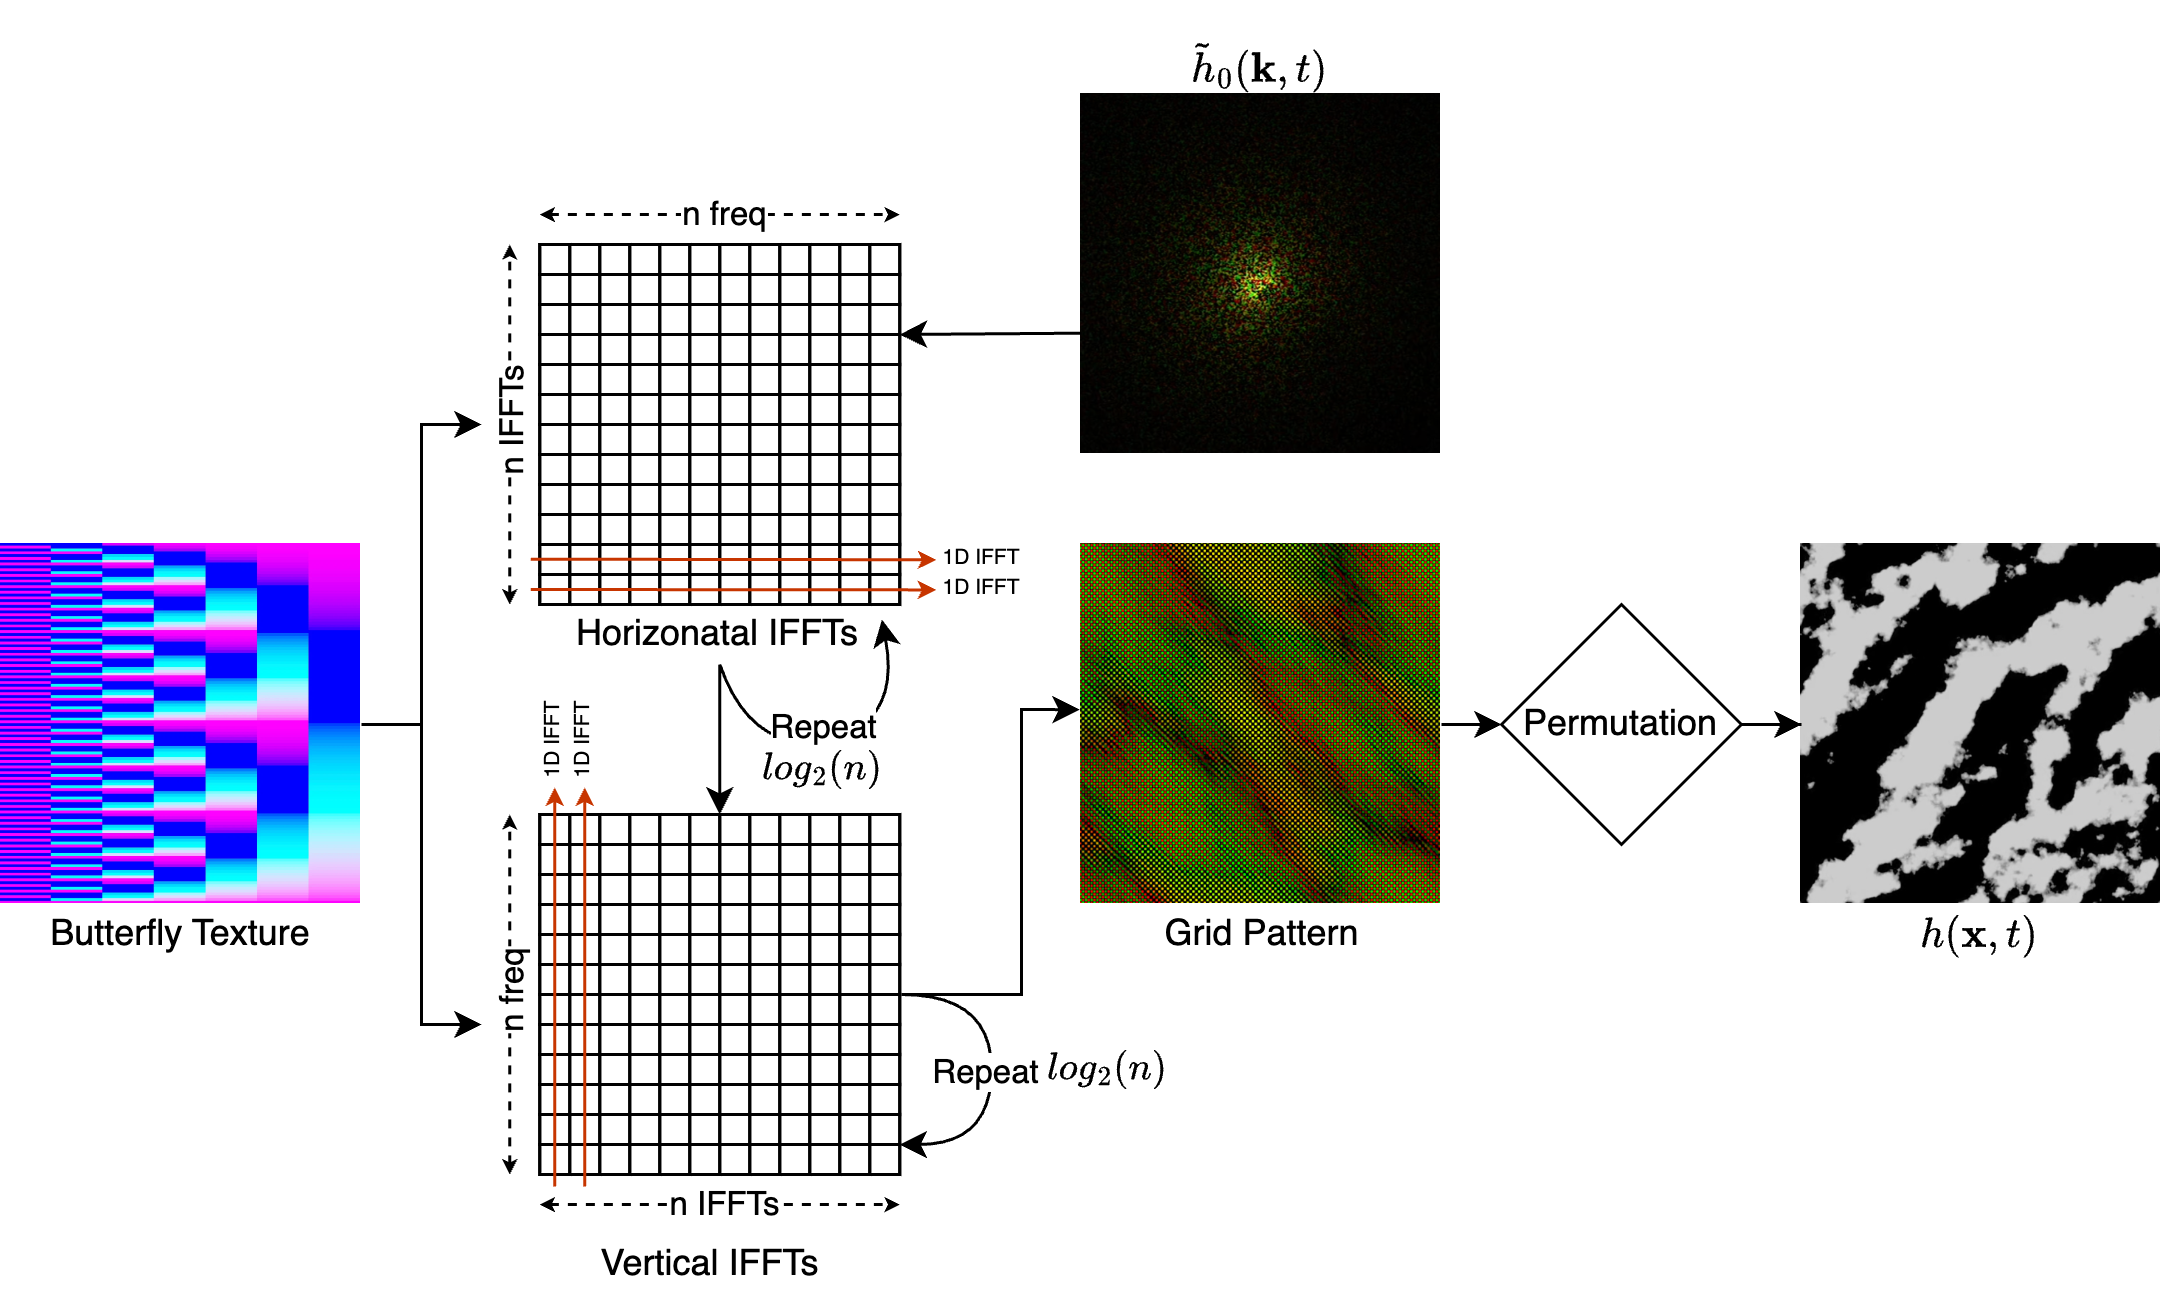
\includegraphics[width=0.7\textwidth]{"images/ifft_algorithm.png"}
    \captionof{figure}{IFFT Algorithm}
    \label{fig:ifft_algorithm}
\end{minipage}

\section{Ocean Geometry}
\subsection{Spectrum Generation}

% Table
\begin{table}[H]
    \centering
    \begin{tabular}{|c|c|}
        \hline
        \textbf{Symbol} & \textbf{Meaning} \\
        \hline
        $S(\omega)$ & Non directional wave spectrum \\
        $S(\omega, \theta)$ & Directional wave spectrum\\
        $S(\mathbf{k})$ & Directional wave spectrum\\
        $\mathbf{k}$ & wave vector \\
        $k$ & Magnetude of wave vector\\
        $l$ & Length scale of the ocean\\
        $\omega$ & dispertion relationship (angular frequency)\\
        $U_{10}$ & Wind speed at 10m above the sea level\\
        $F$ & Fetch (Disntance from lee shore)\\
        $\theta_{\text{wind}}$ & Wind angle\\
        $\lambda$ & Choppy factor\\
        \hline
    \end{tabular}
    \caption{Deffinition Table}
    \label{table:deffinition_table}
\end{table}

Spectrums are responsable for whole look of the ocean. It's importatnt to pick the one that is based on real world data to make our ocean look realistic.
Initialy, Tessendorf spectrum \ref{eq:tessendorf_spectrum} was implemented as it was straight forward to implement. However, it didn't produce satisfying results, as waves didn't seem to transfer energy in convincing way, waves didn't seem to follow wave direction and it was hard to have artistic control over the ocean.

\begin{minipage}{1\textwidth}
    \centering
    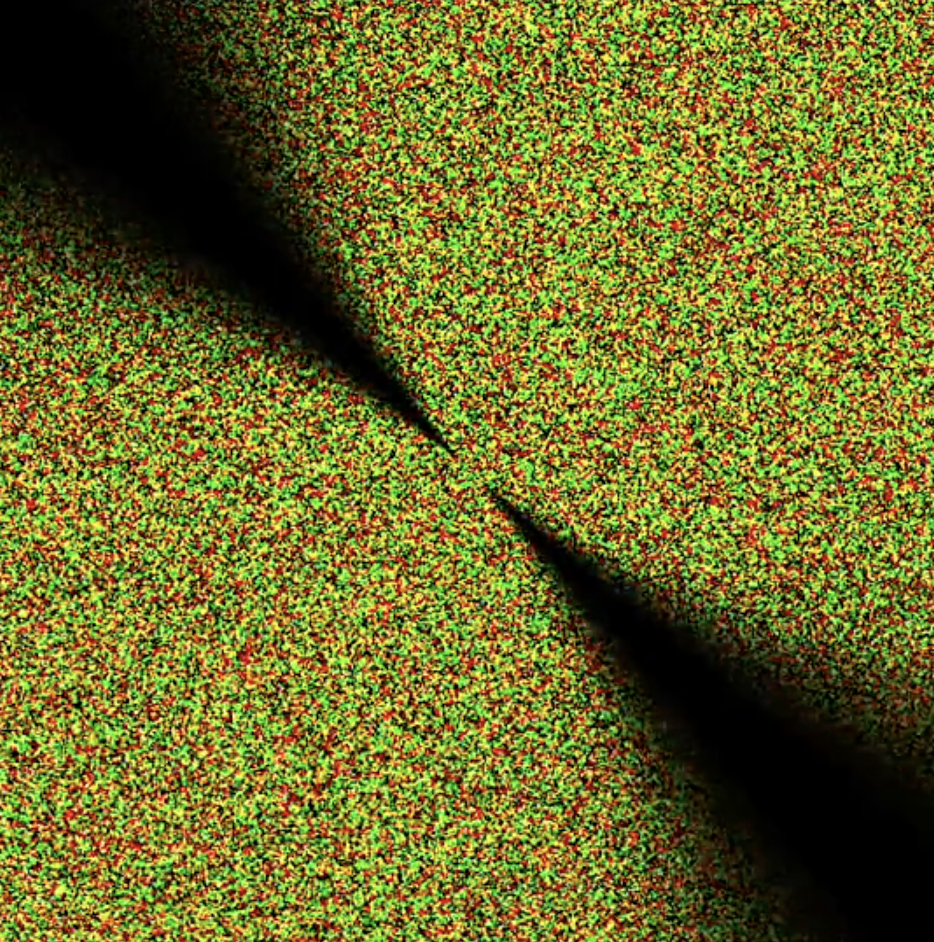
\includegraphics[width=0.4\textwidth]{"images/phillips_spectrum.png"}
    \captionof{figure}{Jerry Tessendorf's Spectrum}
    \label{fig:phillips_spectrum}
\end{minipage}

Therefore, TMA spectrum \ref{eq:tma_spectrum_k} was implemented.

$$
    S_{\text{TMA}}(\mathbf{k}) = 2S_{\text{TMA}}(\omega, h) \cdot \frac{d\omega}{dk} / k \cdot \Delta k_x \cdot \Delta k_y
$$
where $\mathbf{k} = (k_x, k_y)$, $k_x = 2 * \pi (x_x - n/2)/ l$, $k_y = 2 * \pi (x_y - n/2)/ l$, $l$ is the the length scale of the ocean, 
and $\mathbf{x} = (x_x, x_y)$ is current position in the texture. 

This spectrum resulted in more relistic looking ocean with intuitive controls: fetch, wind speed, wind angle, depth. Moreover, it didn't require any efort to make the ocean look relistic and it just worked out of the box.
\begin{minipage}{1\textwidth}
    \centering
    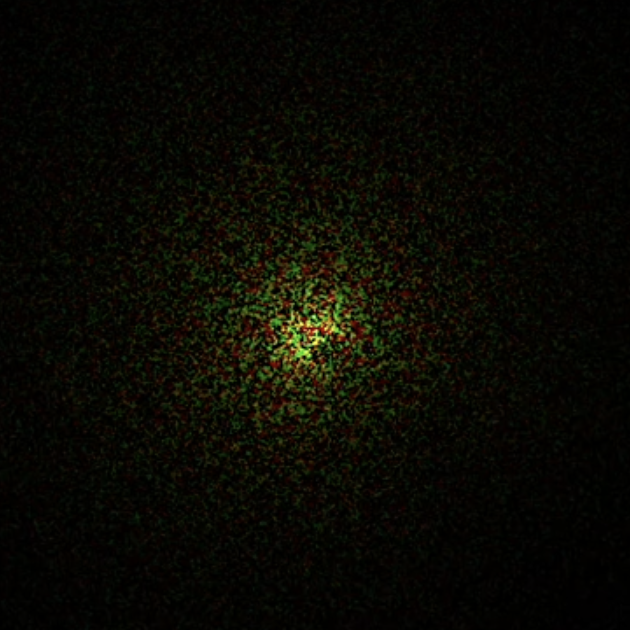
\includegraphics[width=0.40\textwidth]{"images/tma_spectrum.png"}
    \captionof{figure}{TMA spectrum, Frequency Domain \\ (100x for better visibility)}
    \label{fig:tma_spectrum}
\end{minipage}

\subsection{Height Map Generation}

To generate height map, firstlly we need to have fourier amplitudes as shown in \ref{eq:fouier_amplitudes}, where $P_h$ is TMA Spectrum $S_{TMA}(\mathbf{k})$.
For the next step we need to add fourier amplitude and it's complex conjugate to produce "produce waves towards and against the wave direction when propagating"\cite{horvath2015}.
In our luck we don't need to recalculate complex conjugate as fourier series are symetric, so we can just mirror the amplitudes:
\begin{equation}
    \tilde{h}^{*}_0 = T_{h_0}(x^{*}, y^{*})
\end{equation}
where $T_{h_0}(x, y)$ is fourier amplitude in precomputed texture at $x^{*} = (n - x) \text{ mod } n$, $y^{*} = (n - y) \text{ mod } n$, $(x, y)$ is current position in the texture.

By having combined amplitudes \ref{eq:combined_amplitudes} we can perform IFFT as shown in \ref{fig:ifft_algorithm} to produce height map.
\begin{minipage}{1\textwidth}
    \centering
    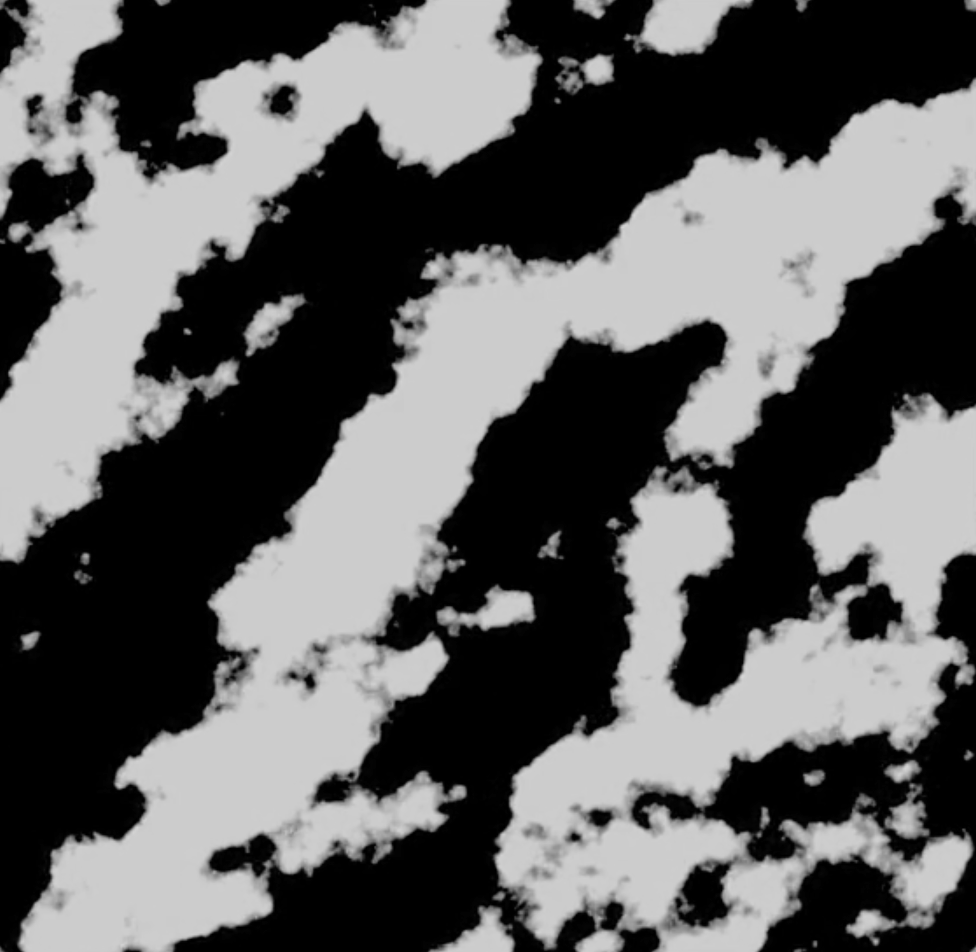
\includegraphics[width=0.40\textwidth]{"images/tma_height.png"}
    \captionof{figure}{Height Map using $S_{\text{TMA}}$}
    \label{fig:tma_height_map}
\end{minipage}

\subsection{Normal Map Generation}
Latter we will need extra information about the ocean to calculate ocean shading. Therefore, we need to calculate normal map. Normal map is perpendicular direction to the surface of the ocean.
To calculate normal map we need to calculate gradient, which is derivative of the height map. According to \cite{tessendorf2004} the derivative is:
\begin{equation}
    \epsilon(\textbf{x}, t) = i\textbf{k} \tilde{h}(\textbf{k}, t)
\end{equation}
Then we need to perform IFFT \ref{fig:ifft_algorithm} to get normal map in the time domain.

\begin{minipage}{1\textwidth}
    \centering
    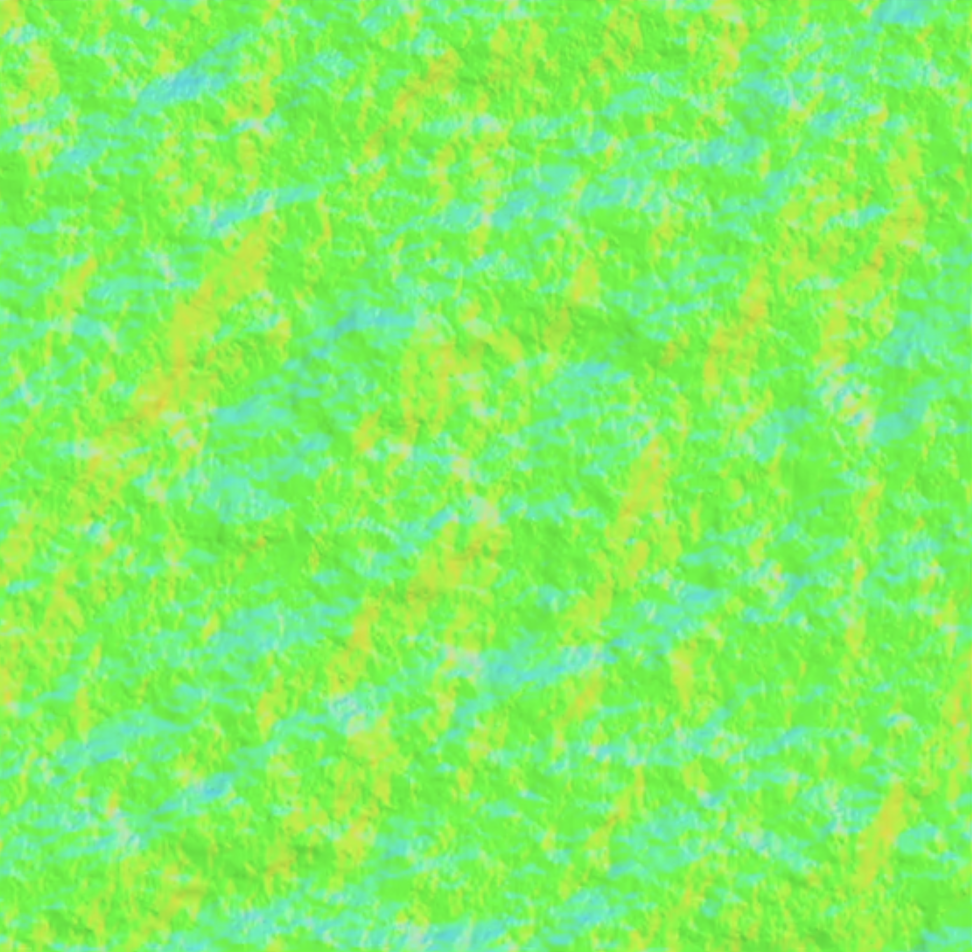
\includegraphics[width=0.40\textwidth]{"images/tma_normal.png"}
    \captionof{figure}{Normal Map using $S_{\text{TMA}}$}
    \label{fig:tma_normal_map}
\end{minipage}

\subsection{Choppy Waves}
Currentlly, when rendering ocean it looks too smooth \ref{fig:ocean_no_choppy} and lacks choppiness.

\begin{minipage}{1\textwidth}
    \centering
    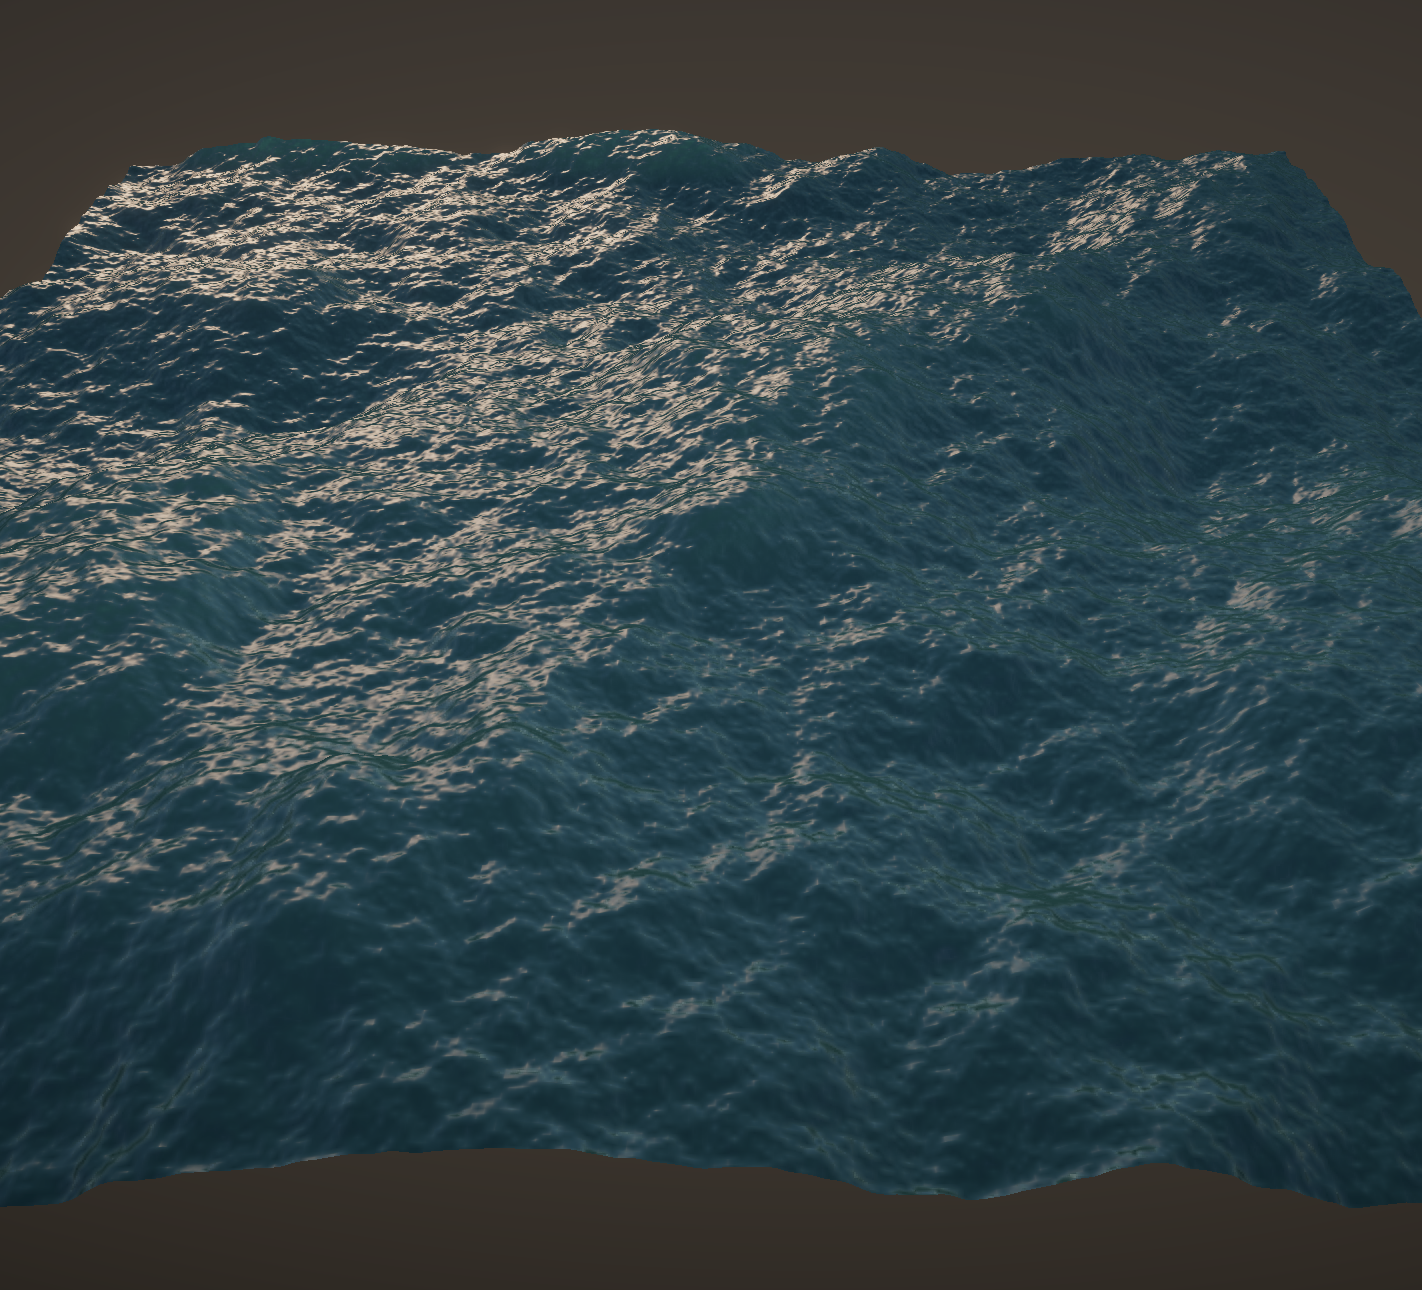
\includegraphics[width=0.40\textwidth]{"images/rendered_height_no_coppy.png"}
    \captionof{figure}{Ocean without Choppy Waves}
    \label{fig:ocean_no_choppy}
\end{minipage}

To make waves choppy we need to introduce horizotal displacement. This will not only make waves more chopy but also make energy transfer between waves more relistic. Following formula from \cite[J. Tessendorf]{tessendorf2004} we can calculate horizontal displacement:
\begin{equation}
    \mathbf{D}_{\text{hori}}(\textbf{x}, t) = -i\frac{\mathbf{k}}{k}\tilde{h(\mathbf{k}, t)}
\end{equation}
Using this horizotal displacement we can displace our verticies:
\begin{equation}
    \mathbf{x} + \lambda \mathbf{D}_{\text{hori}}(\textbf{x}, t)
\end{equation}
, where $\lambda$ is "choppy factor".
Once again we need to perform IFFT \ref{fig:ifft_algorithm} to get horizontal displacement in the time domain.

\begin{minipage}{1\textwidth}
    \centering
    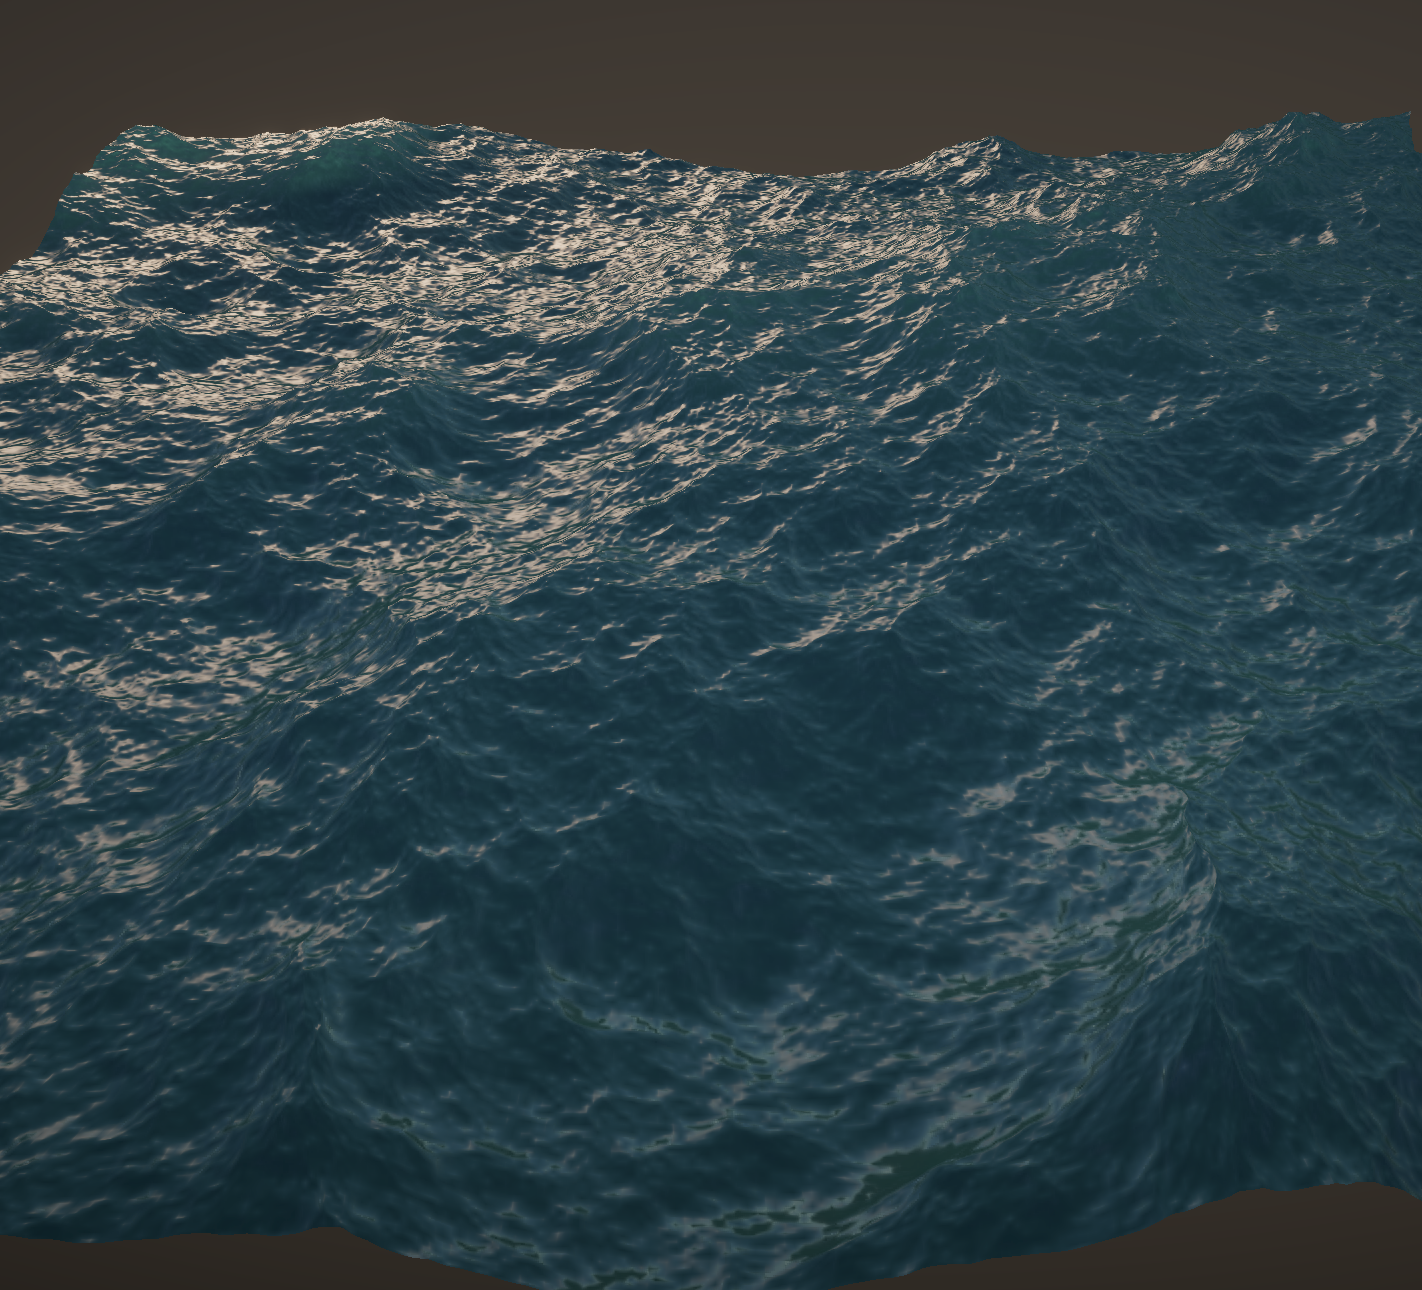
\includegraphics[width=0.40\textwidth]{"images/rendered_height_choppy.png"}
    \captionof{figure}{Ocean with Choppy Waves}
    \label{fig:ocean_choppy}
\end{minipage}

\section{Ocean Shading}

\begin{table}[H]
    \centering
    \begin{tabular}{|c|c|c|}
        \hline
        \textbf{Symbol} & \textbf{Parameter} \\
        \hline
        $L_a$ & Ambient Light \\
        $L_ss$ & Subsurface Scatter Light\\
        $L_s$ & Specular Light\\
        $L_r$ & Enviroment Reflection\\
        $N$ & Normal \\
        $D_s$ & Sun Direction \\
        $D_v$ & View Direction \\
        $C_a$ & Ambient Light Color \\
        $C_l$ & Light Color \\
        $C_b$ & Air Bubble Color \\
        $C_{ws}$ & Water Scattering Color \\
        $H$ & Ocean Height \\
        $F$ & Fresnel Effect \\
        $\rho_a$ & Air Bubble Density \\
        $k_a$ & Ambient Light Intensity \\
        $k_{ss_1}$ & Subsurface Scattering Intensity \\
        $k_{ss_2}$ & Subsurface Scattering Intensity \\
        \hline
    \end{tabular}
    \caption{Lighting Parameters}
    \label{table:lighting_parameters}
\end{table}

\subsection{Lighting Model}

\subsubsection{Output}
[MENTION PHON SHADING DISCCUSED IN BACKGROUND RESERCH]

Our lighting model, as depicted in Equation \ref{eq:light_model}, comprises four integral components: ambient light, subsurface scattering, specular light, and environmental reflection. The culmination of these components results in the final output, as illustrated in Figure \ref{fig:output_light}
\begin{equation}
    L = L_a + L_{ss} + L_s + L_r
    \label{eq:light_model}
\end{equation}
\begin{minipage}{1\textwidth}
    \centering
    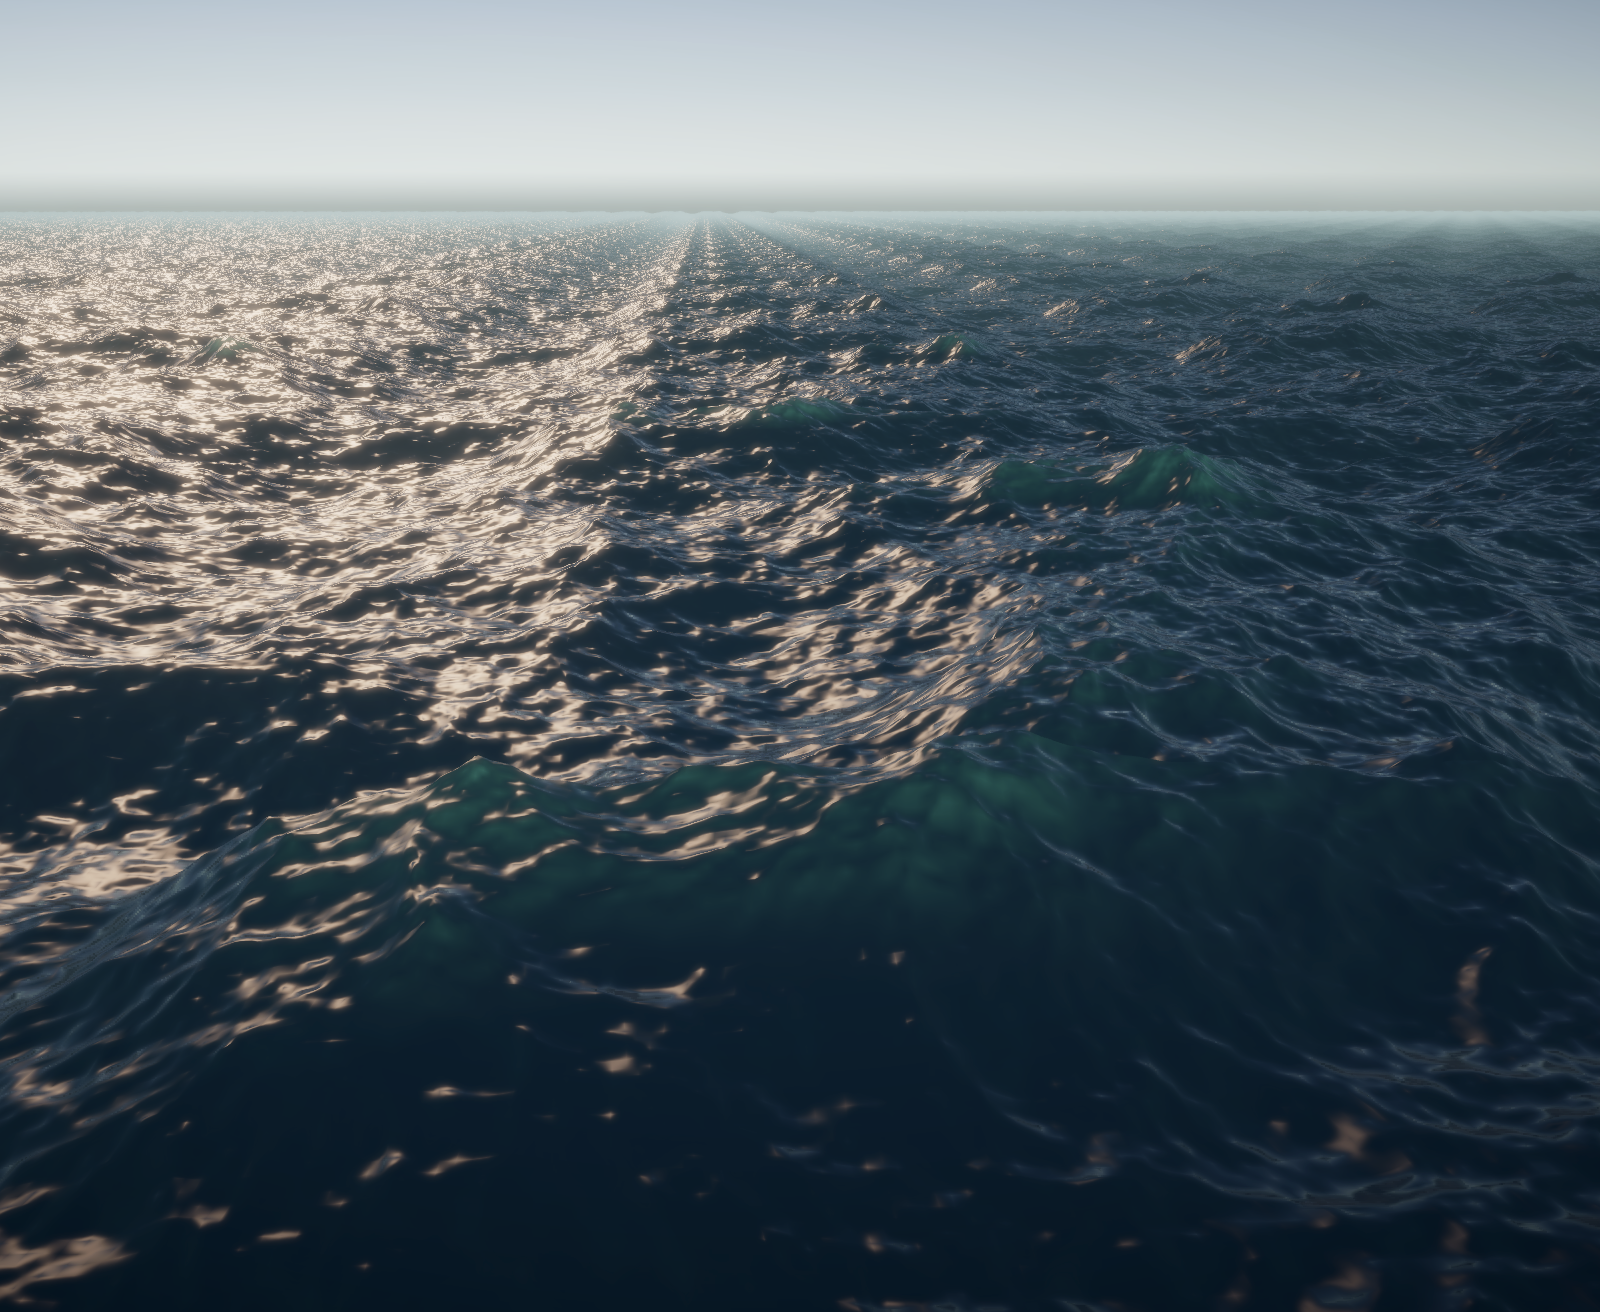
\includegraphics[width=0.50\textwidth]{"images/output_light.png"}
    \captionof{figure}{Finall Shader Output}
    \label{fig:output_light}
\end{minipage}

\subsubsection{Ambient Light}
Ambient light, a constant illumination that does not depend on the direction of the light source, is the result of light scattering in the environment. For oceanic simulations, we utilize an approximation formula for ambient light derived from the GDC conference \cite{mark2021}: 
\begin{equation}
    L_a = k_a N C_a C_l + \rho_a C_b C_l
\end{equation}
\begin{minipage}{1\textwidth}
    \centering
    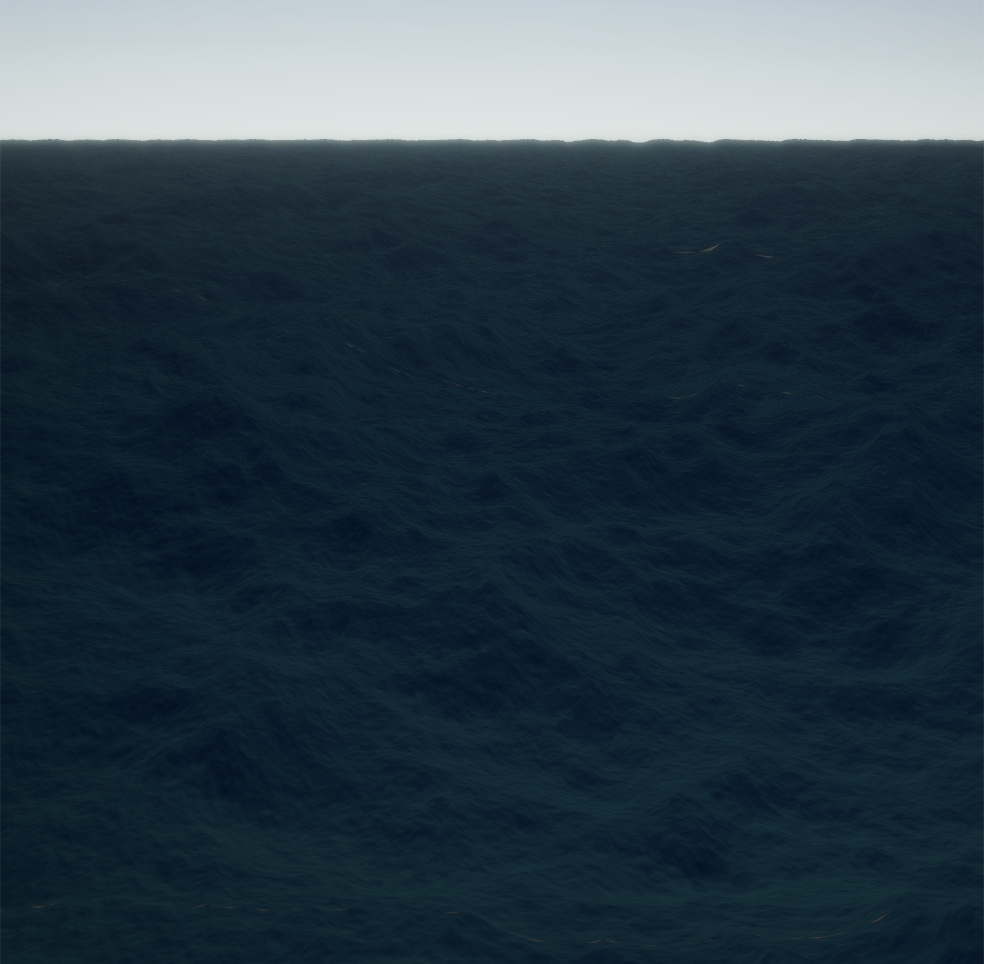
\includegraphics[width=0.40\textwidth]{"images/ambient_light.png"}
    \captionof{figure}{Ambient Light}
    \label{fig:ambient_light}
\end{minipage}

\subsubsection{Fresnel Effect}
The Fresnel effect, a phenomenon where light is more reflective at grazing angles as shown in figure \ref{fig:fresnel_effect}, is crucial for calculations involving specular and reflection:
\begin{equation}
    F = (1 - \max(D_v \cdot N, 0.15))^{5}
\end{equation}
\begin{minipage}{1\textwidth}
    \centering
    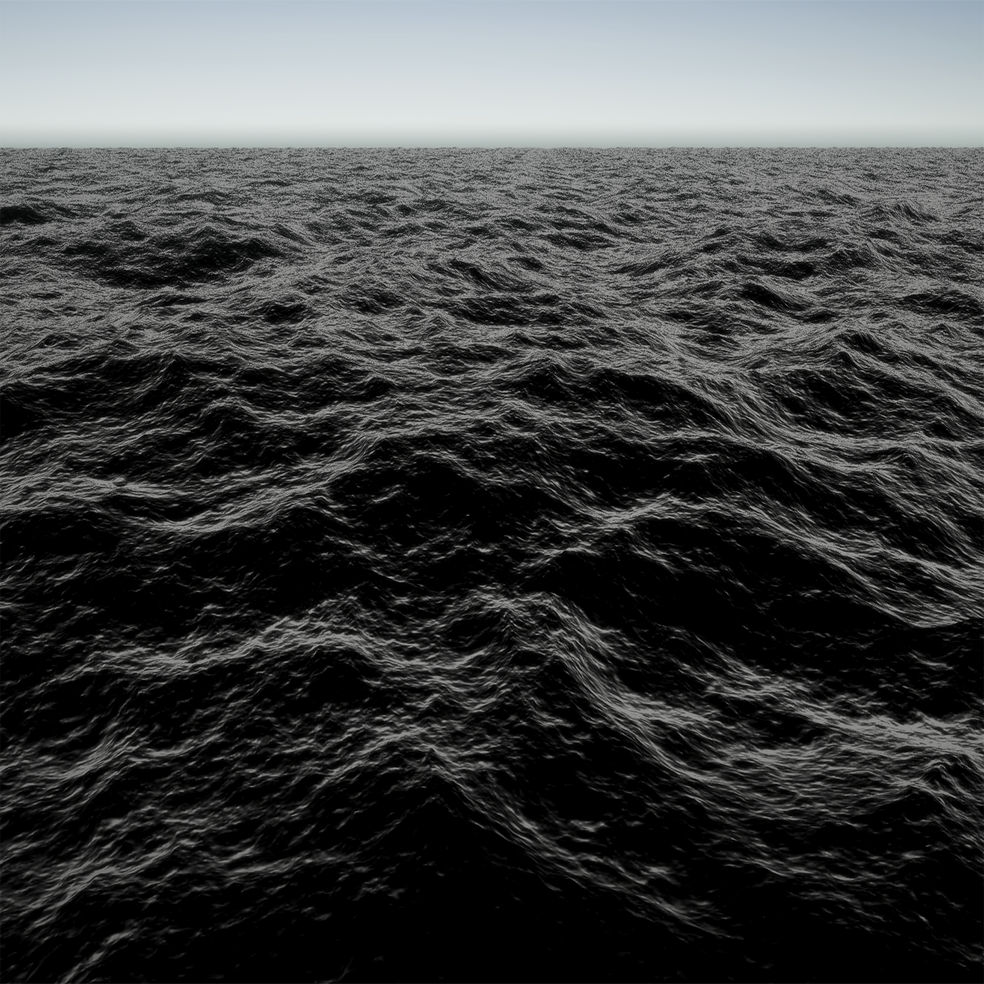
\includegraphics[width=0.40\textwidth]{"images/fresnel.png"}
    \captionof{figure}{Fresnel Effect}
    \label{fig:fresnel_effect}
\end{minipage}

\subsubsection{Subsurface Scattering}

[SAY AS EARLIER MENTIONED]

Subsurface scattering describes the interaction of light when it penetrates an object, in this case, water. While ray tracing would typically be required for realistic results, we can use an approximation from the GDC conference \cite{mark2021} due to the majority of our light being trapped in the ocean, with only light at wave peaks able to escape. 
\begin{equation}
    \begin{split}
        L_{ss} &= (L_{ss_1} + L_{ss_2}) C_{ws} C_l\\
        L_{ss_1} &= k_{ss_1} \max(0, H) ([D_s, -D_v])^{4}(0.5-0.5(D_s \cdot N))^{3}\\
        L_{ss_2} &= k_{ss_2} ([D_V, N])^{2}
    \end{split}
\end{equation}
\begin{minipage}{0.32\textwidth}
    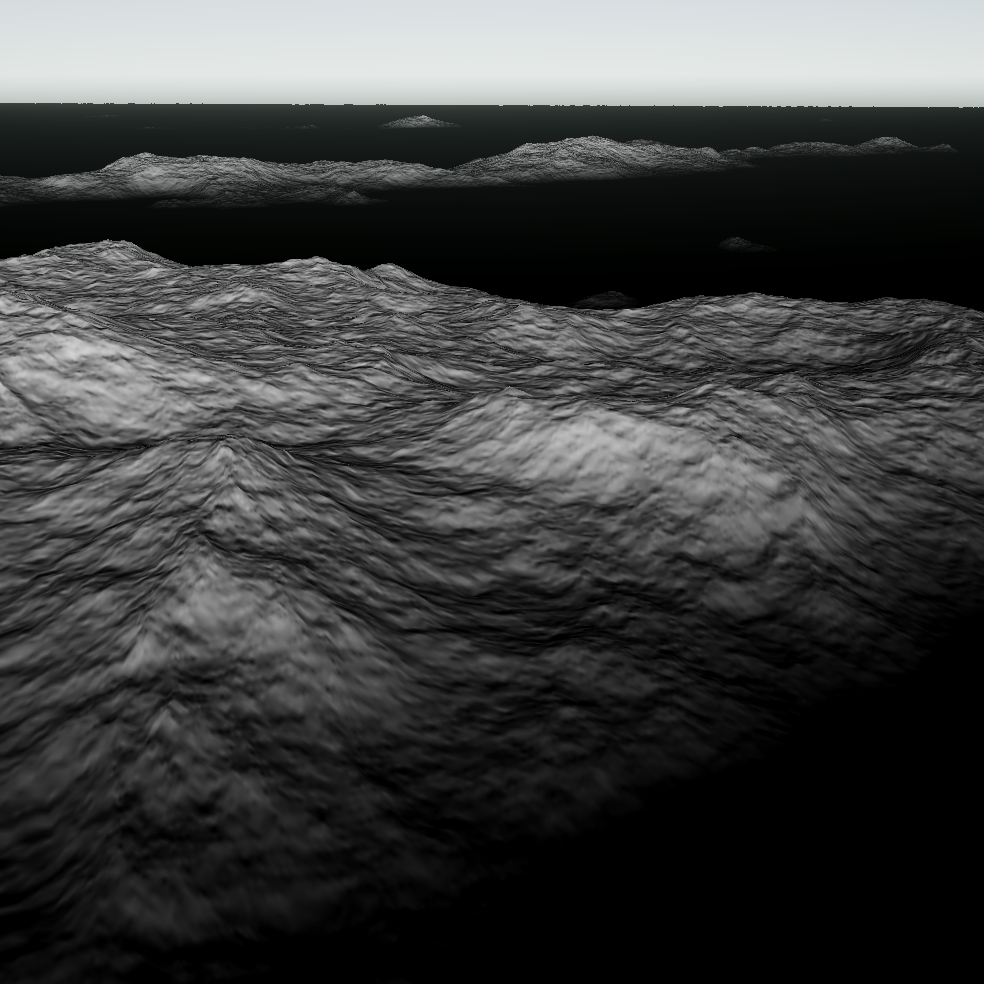
\includegraphics[width=1\textwidth]{"images/ss1_light.png"}
    \captionof{figure}{$L_{ss_1}$}
    \label{fig:lss1_light}
\end{minipage}
\hfill
\begin{minipage}{0.32\textwidth}
    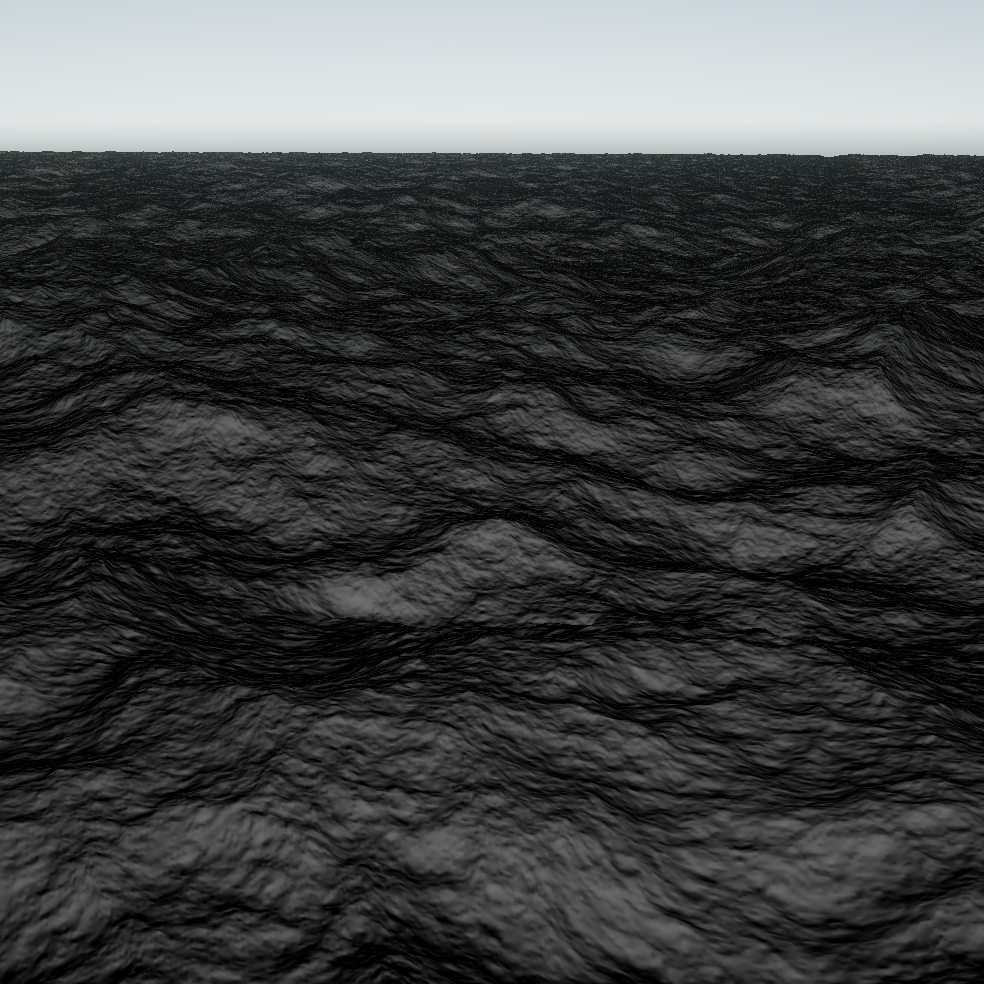
\includegraphics[width=1\textwidth]{"images/ss2_light.png"}
    \captionof{figure}{$L_{ss_2}$}
    \label{fig:lss2_light}
\end{minipage}
\hfill
\begin{minipage}{0.32\textwidth}
    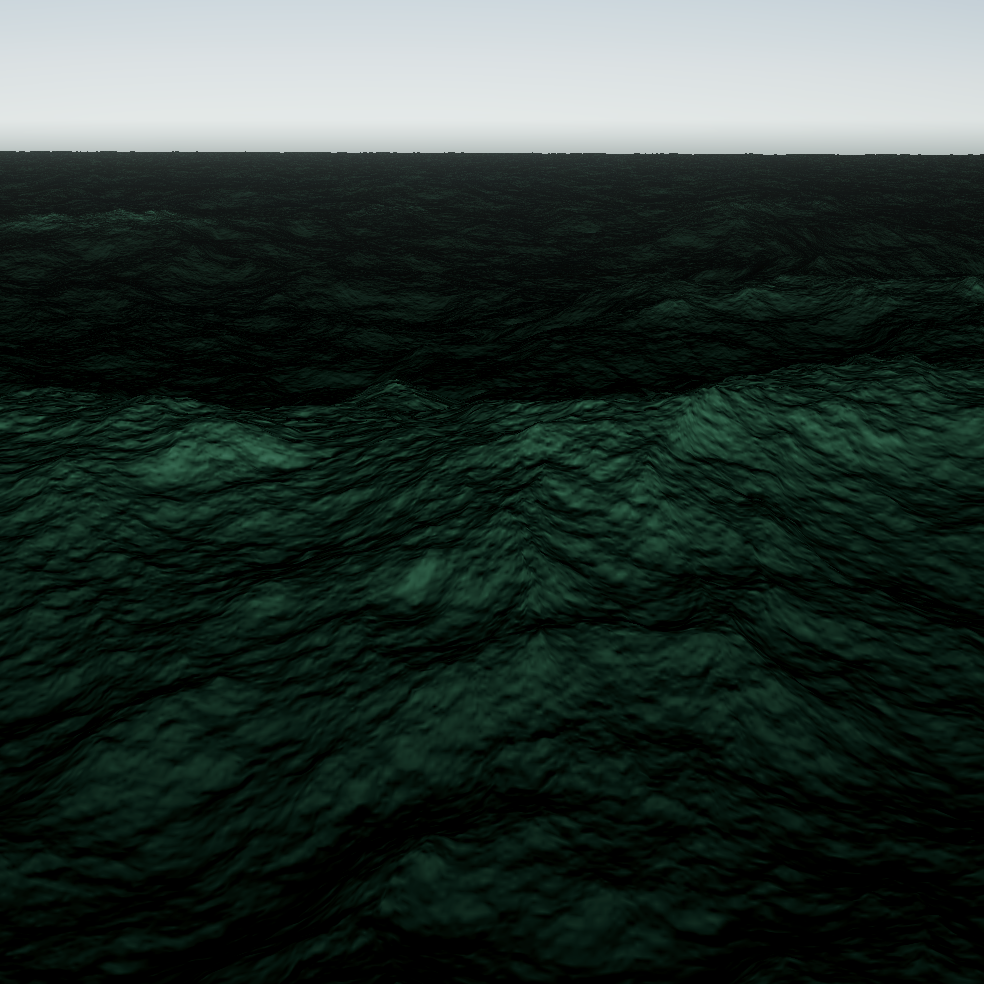
\includegraphics[width=1\textwidth]{"images/ss_light.png"}
    \captionof{figure}{Subsurface Scattering}
    \vspace*{-13pt}
    \label{fig:lss_light}
\end{minipage}

\subsubsection{Specular Reflection}
Specular reflection, the reflection of light from a light source on an object, is a characteristic of shiny objects like metals, plastic, or in our case, water. We employ a simple Phong scattering technique, as shown in Figure \ref{fig:specular_light}, and the formula takes the following form:
\begin{equation}
    \begin{split}
        L_s &= C_l S C_s F\\
        S &= [D_v, D_r]^{\text{Shininess}}\\
        D_r &= \text{reflect}(\text{LightPos}, N)
    \end{split}
\end{equation}
\begin{minipage}{1\textwidth}
    \centering
    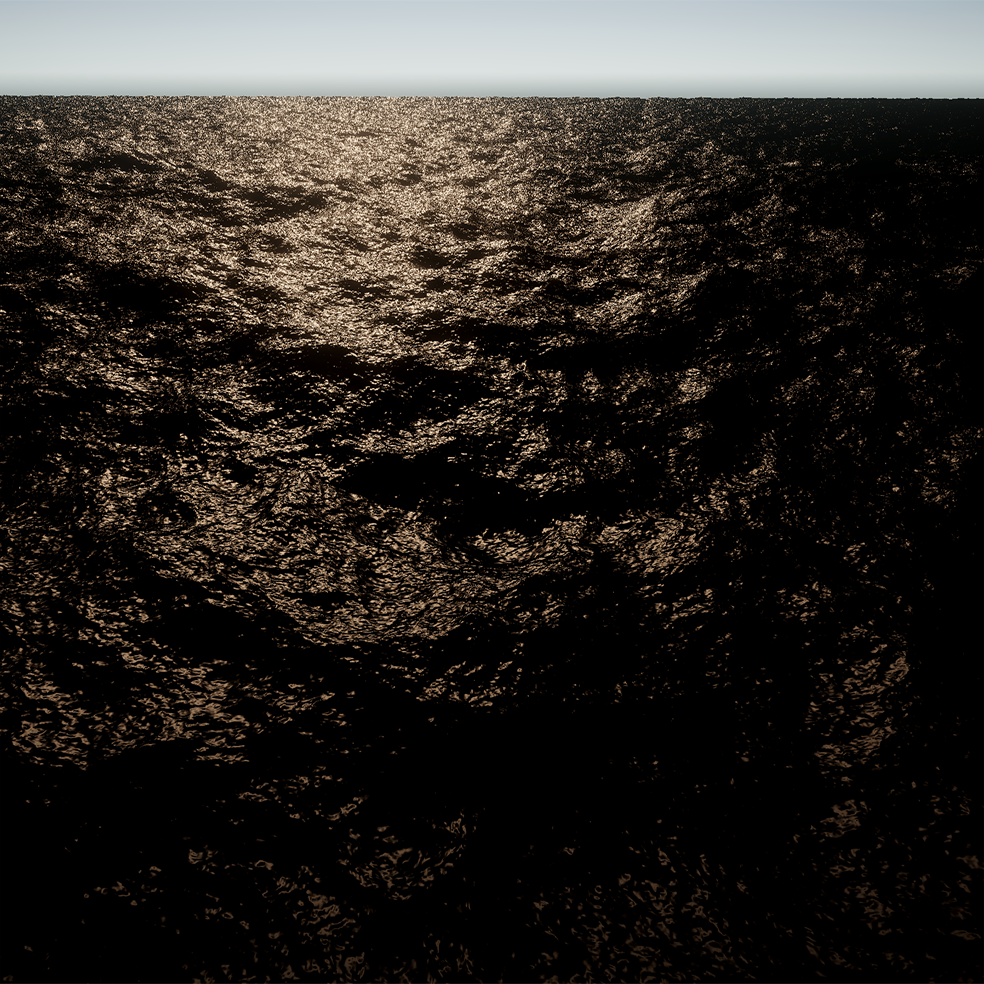
\includegraphics[width=0.45\textwidth]{"images/specular_light.png"}
    \captionof{figure}{Specular Reflection}
    \label{fig:specular_light}
\end{minipage}

\subsubsection{Enviroment Reflection}
In our project, we only consider the reflection of the skybox on the water surface. As per Figure \ref{fig:relfection_light}, we illustrate how skybox reflection operates on a calm ocean surface to better visualize environmental reflection.
\begin{equation}
    \begin{split}
        L_r &= F k_r C_{\text{sky}}\\
        C_{\text{sky}} &= \text{Sky}[\text{reflect}{D_i, N}]
    \end{split}
\end{equation}
\begin{minipage}{1\textwidth}
    \centering
    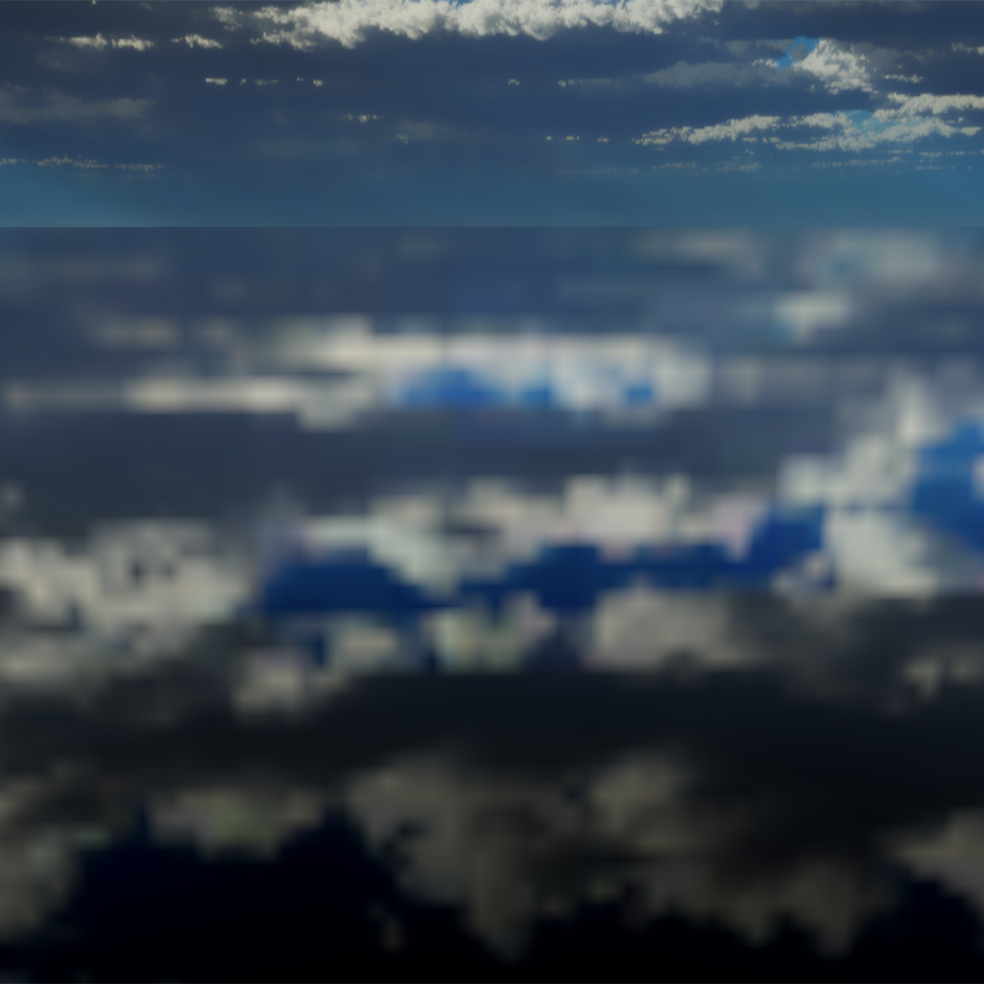
\includegraphics[width=0.45\textwidth]{"images/reflection_light.png"}
    \captionof{figure}{Skybox reflection on calm ocean}
    \label{fig:relfection_light}
\end{minipage}

\subsection{Foam}
\subsubsection{Foam Generation}
\begin{minipage}{1\textwidth}
    \centering
    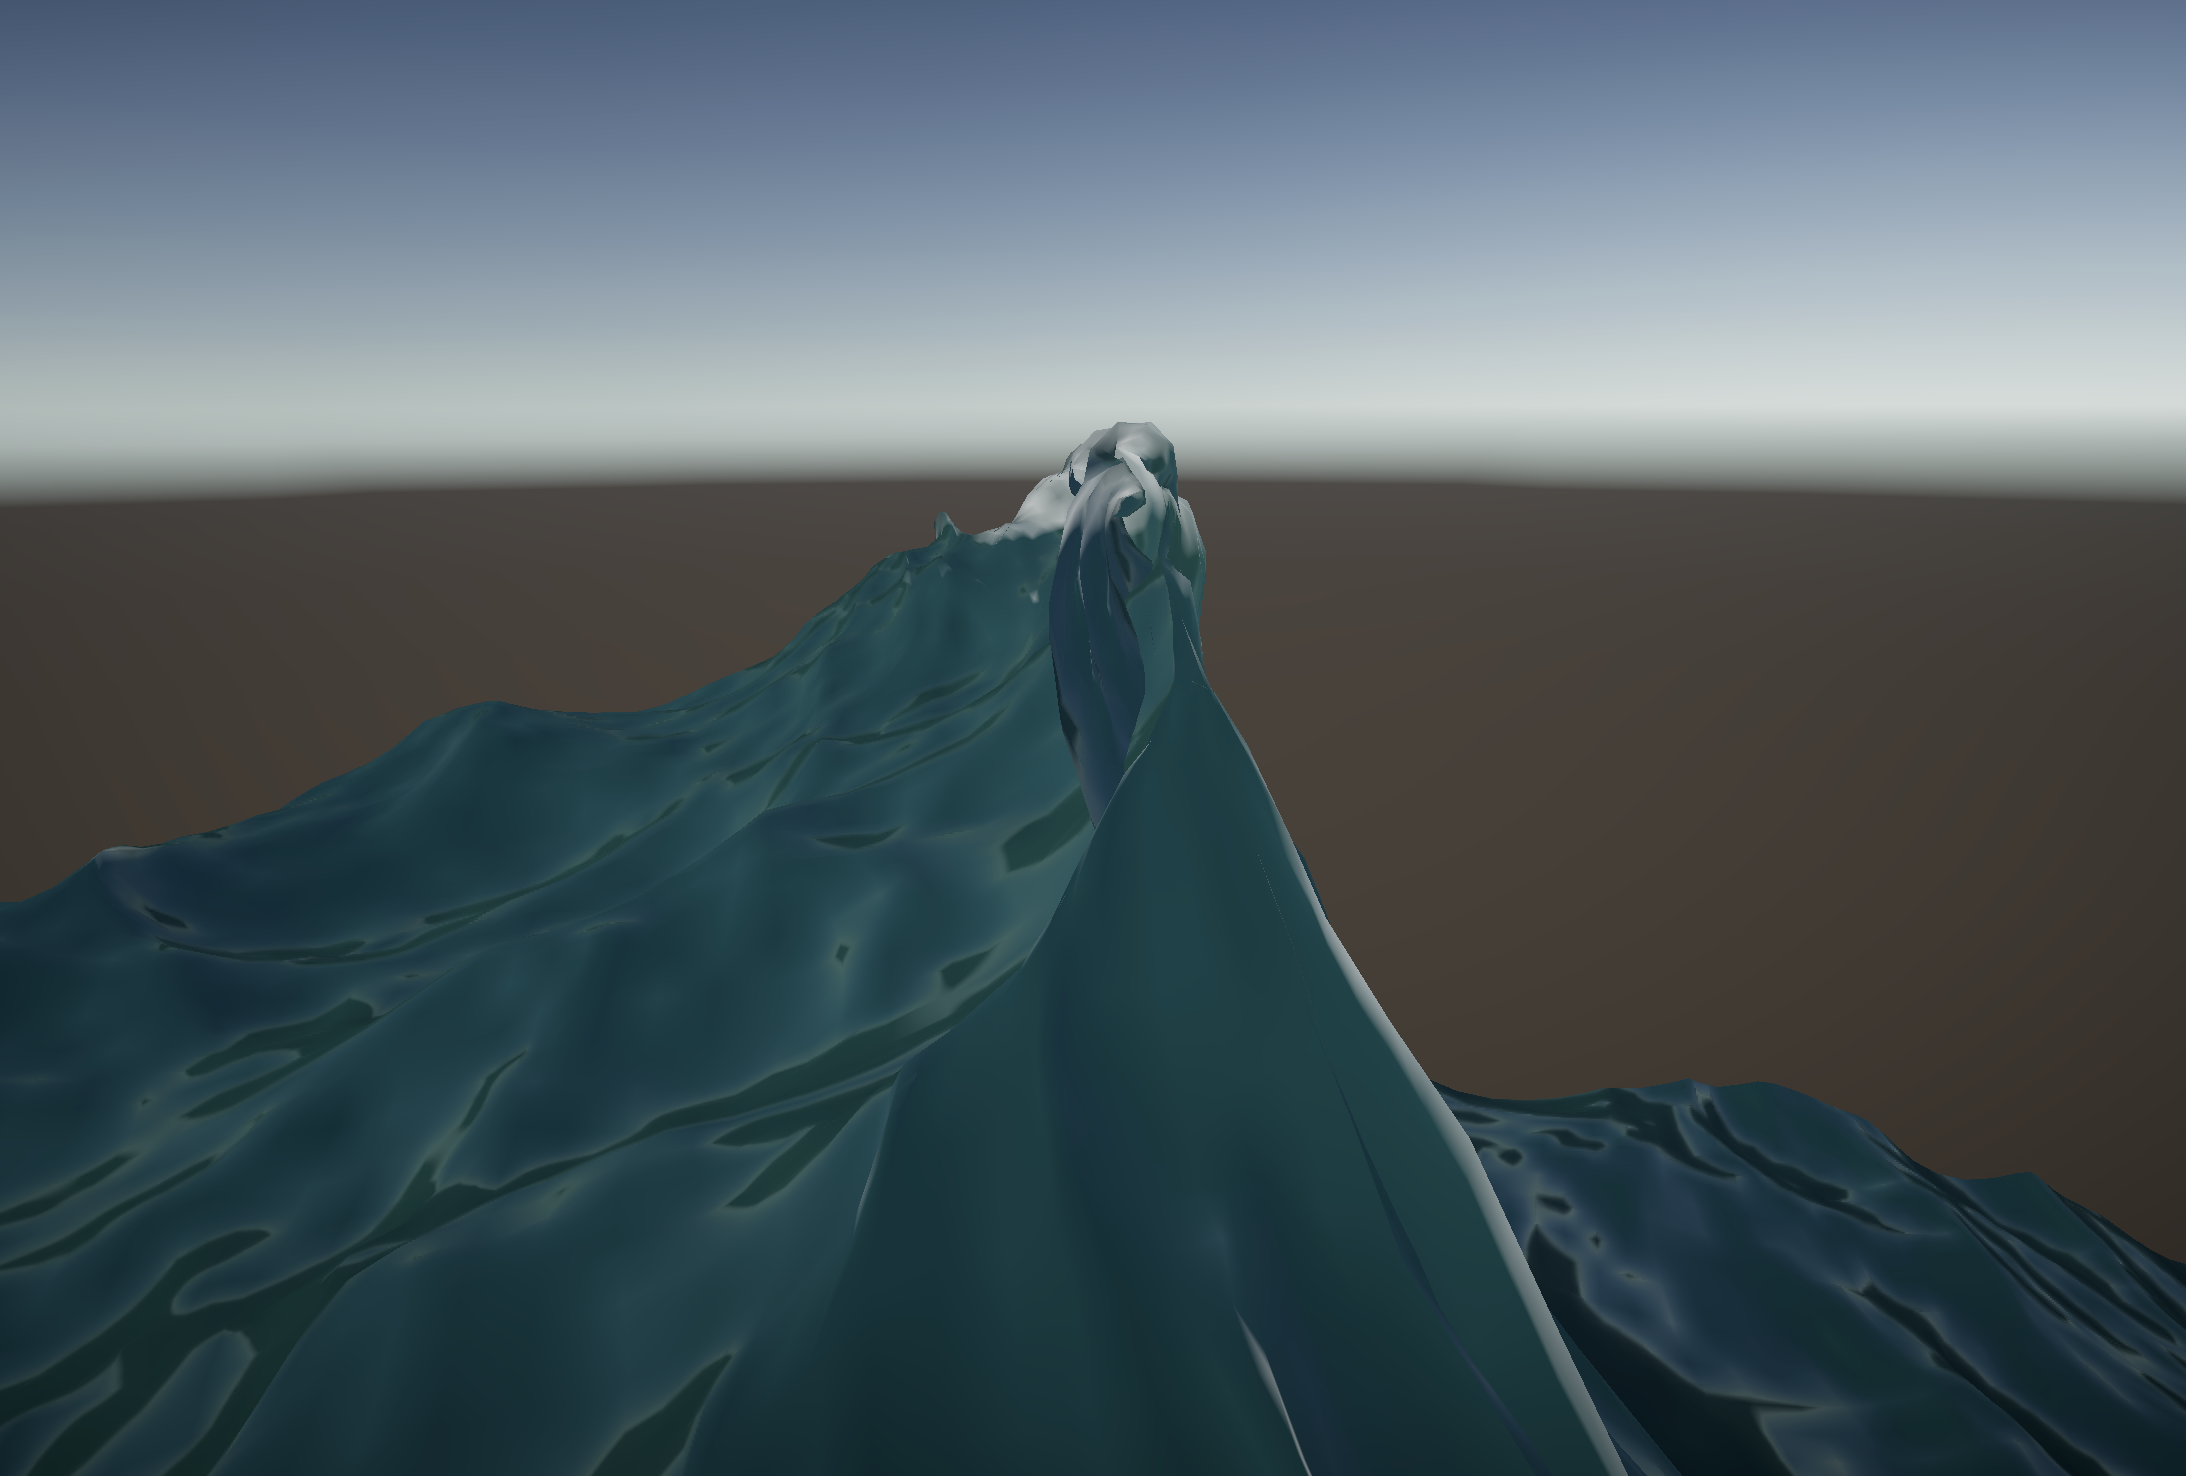
\includegraphics[width=0.50\textwidth]{"images/wave_curl.png"}
    \captionof{figure}{Wave Curl At Wave Peek}
    \label{fig:wave_curl}
\end{minipage}

Ocean foam is a salient and realistic feature of the ocean, contributing to its distinct and authentic appearance. The primary occurrence of foam is observed during wave crashes, a phenomenon facilitated by horizontal displacement. This can be visually discerned at the peaks of waves where the water curls up, as illustrated in Figure \ref{fig:wave_curl}. In essence, our horizontal transformation undergoes an inversion.

As proposed by Tessendorf \cite{tessendorf2001}, the rendering of foam can be achieved by calculating the determinant of the Jacobian matrix for horizontal displacement, which helps identify these inversions. In our ocean simulation, the Jacobian matrix provides insights into the changes over the x and z axes. When determinant of the Jacobian matrix is bellow zero the "wave crash" happens:

\begin{equation}
    \text{Det}(\mathbf{x}) = J_{xx} + J_{yy} - J_{xy} J_{yx}
\end{equation}
where,
\begin{equation}
    J(\mathbf{x}) = 
    \begin{bmatrix} 
        1 + \lambda\frac{\partial D_x(\mathbf{x})}{\partial x} & 1 + \lambda\frac{\partial D_x(\mathbf{x})}{\partial y} \\
        1 + \lambda\frac{\partial D_y(\mathbf{x})}{\partial x} & 1 + \lambda\frac{\partial D_y(\mathbf{x})}{\partial y} 
    \end{bmatrix} 
\end{equation}
in this case $J_{xy} = J_{yx}$.

\begin{minipage}{1\textwidth}
    \centering
    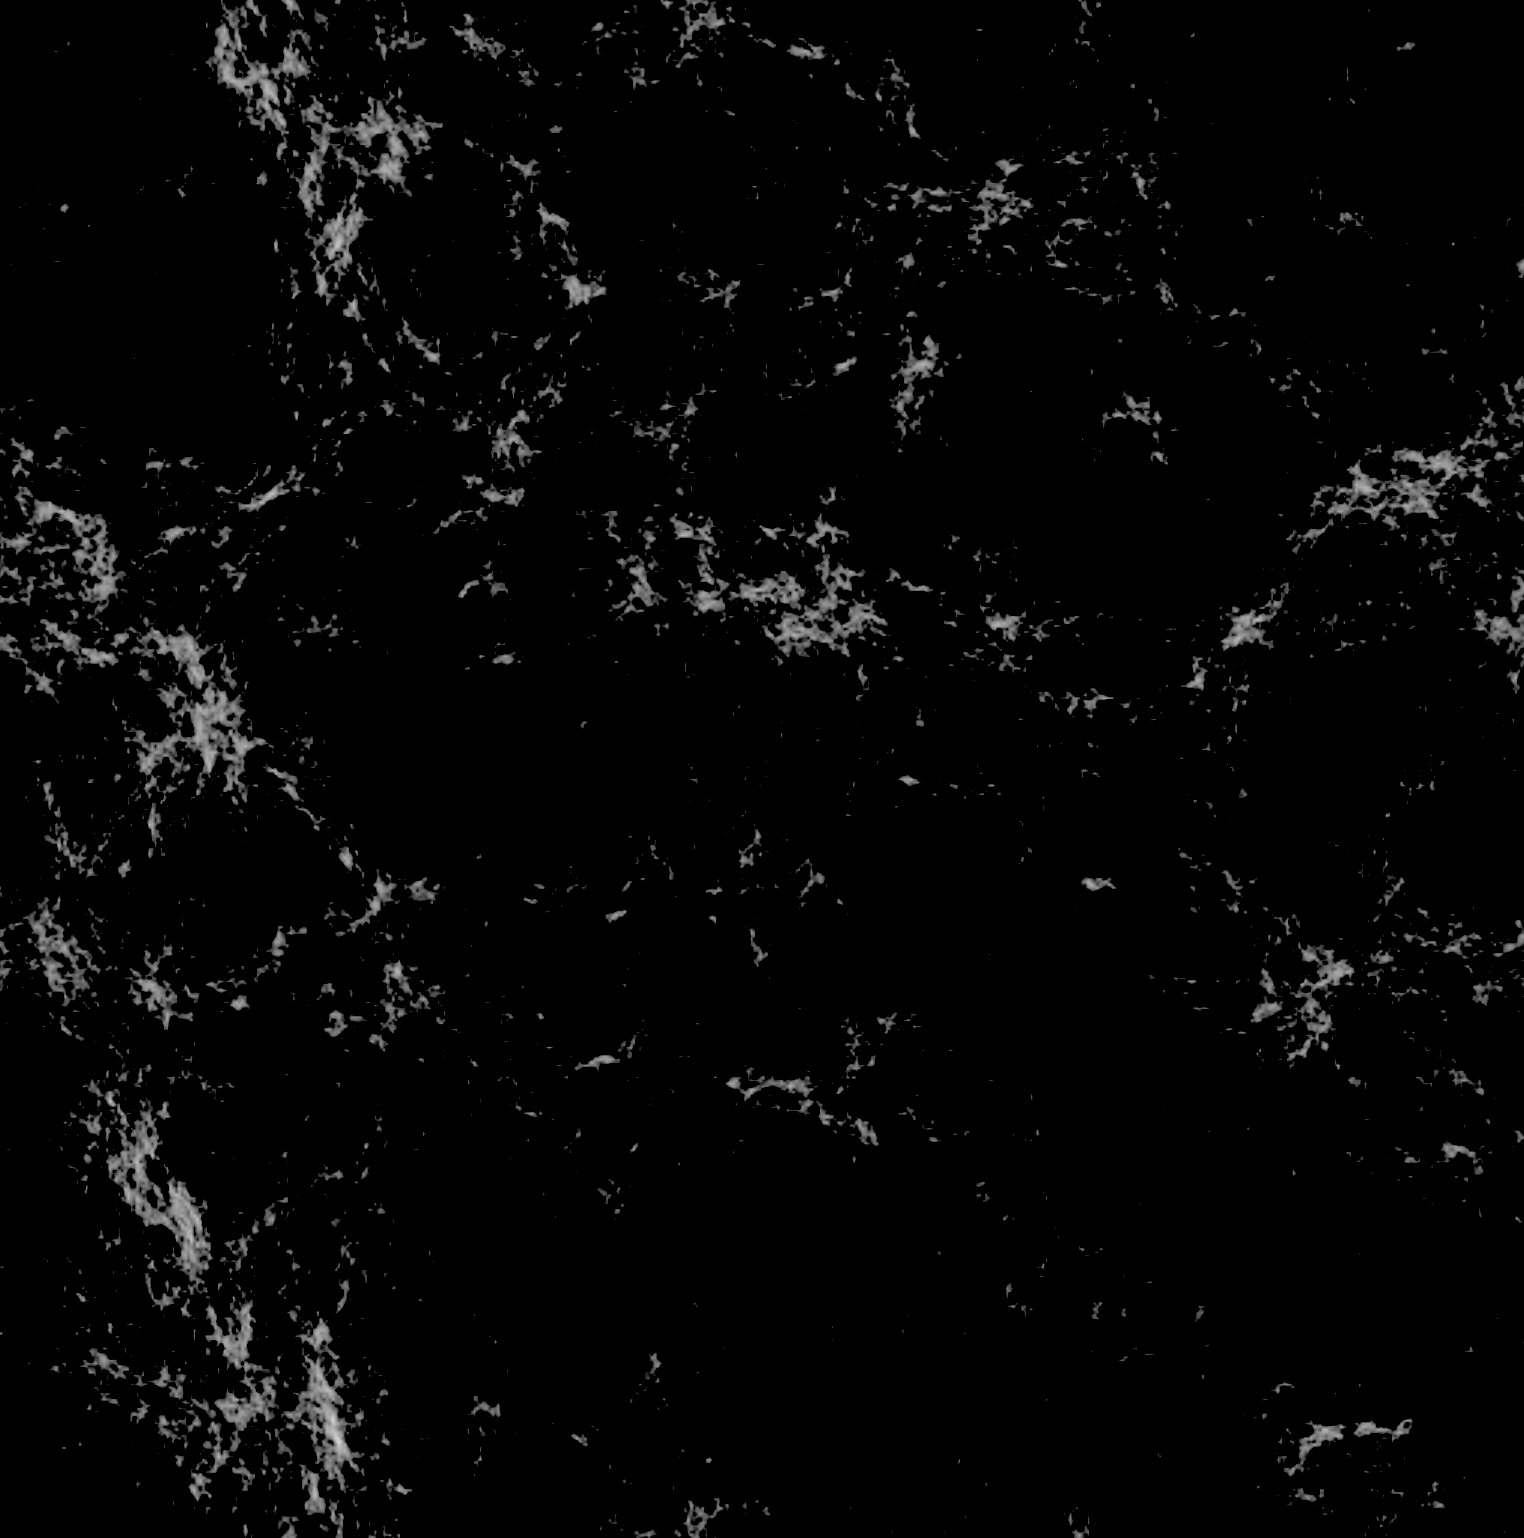
\includegraphics[width=0.40\textwidth]{"images/foam_texture.png"}
    \captionof{figure}{Foam Texture}
    \label{fig:foam_texture}
\end{minipage}

\subsubsection{Foam Accumilation}
Curretlly the foam apears and diasapears quicly, however in real life the foam accumilates and disapears over time.
We can introduce foam accumilation by compering previous and current foam values:
\begin{lstlisting}[caption={Foam Accumilation}, frame=single, numberstyle=\small\color{gray}, captionpos=b]
    float accumulation = 
    LastFoamValue - FoamDecay * DeltaTime / max(currentFoam, 0.5);
    float foam = max(accumulation, currentFoam);
\end{lstlisting}
This results in pleasing foam accumilation:

\begin{minipage}{1\textwidth}
    \centering
    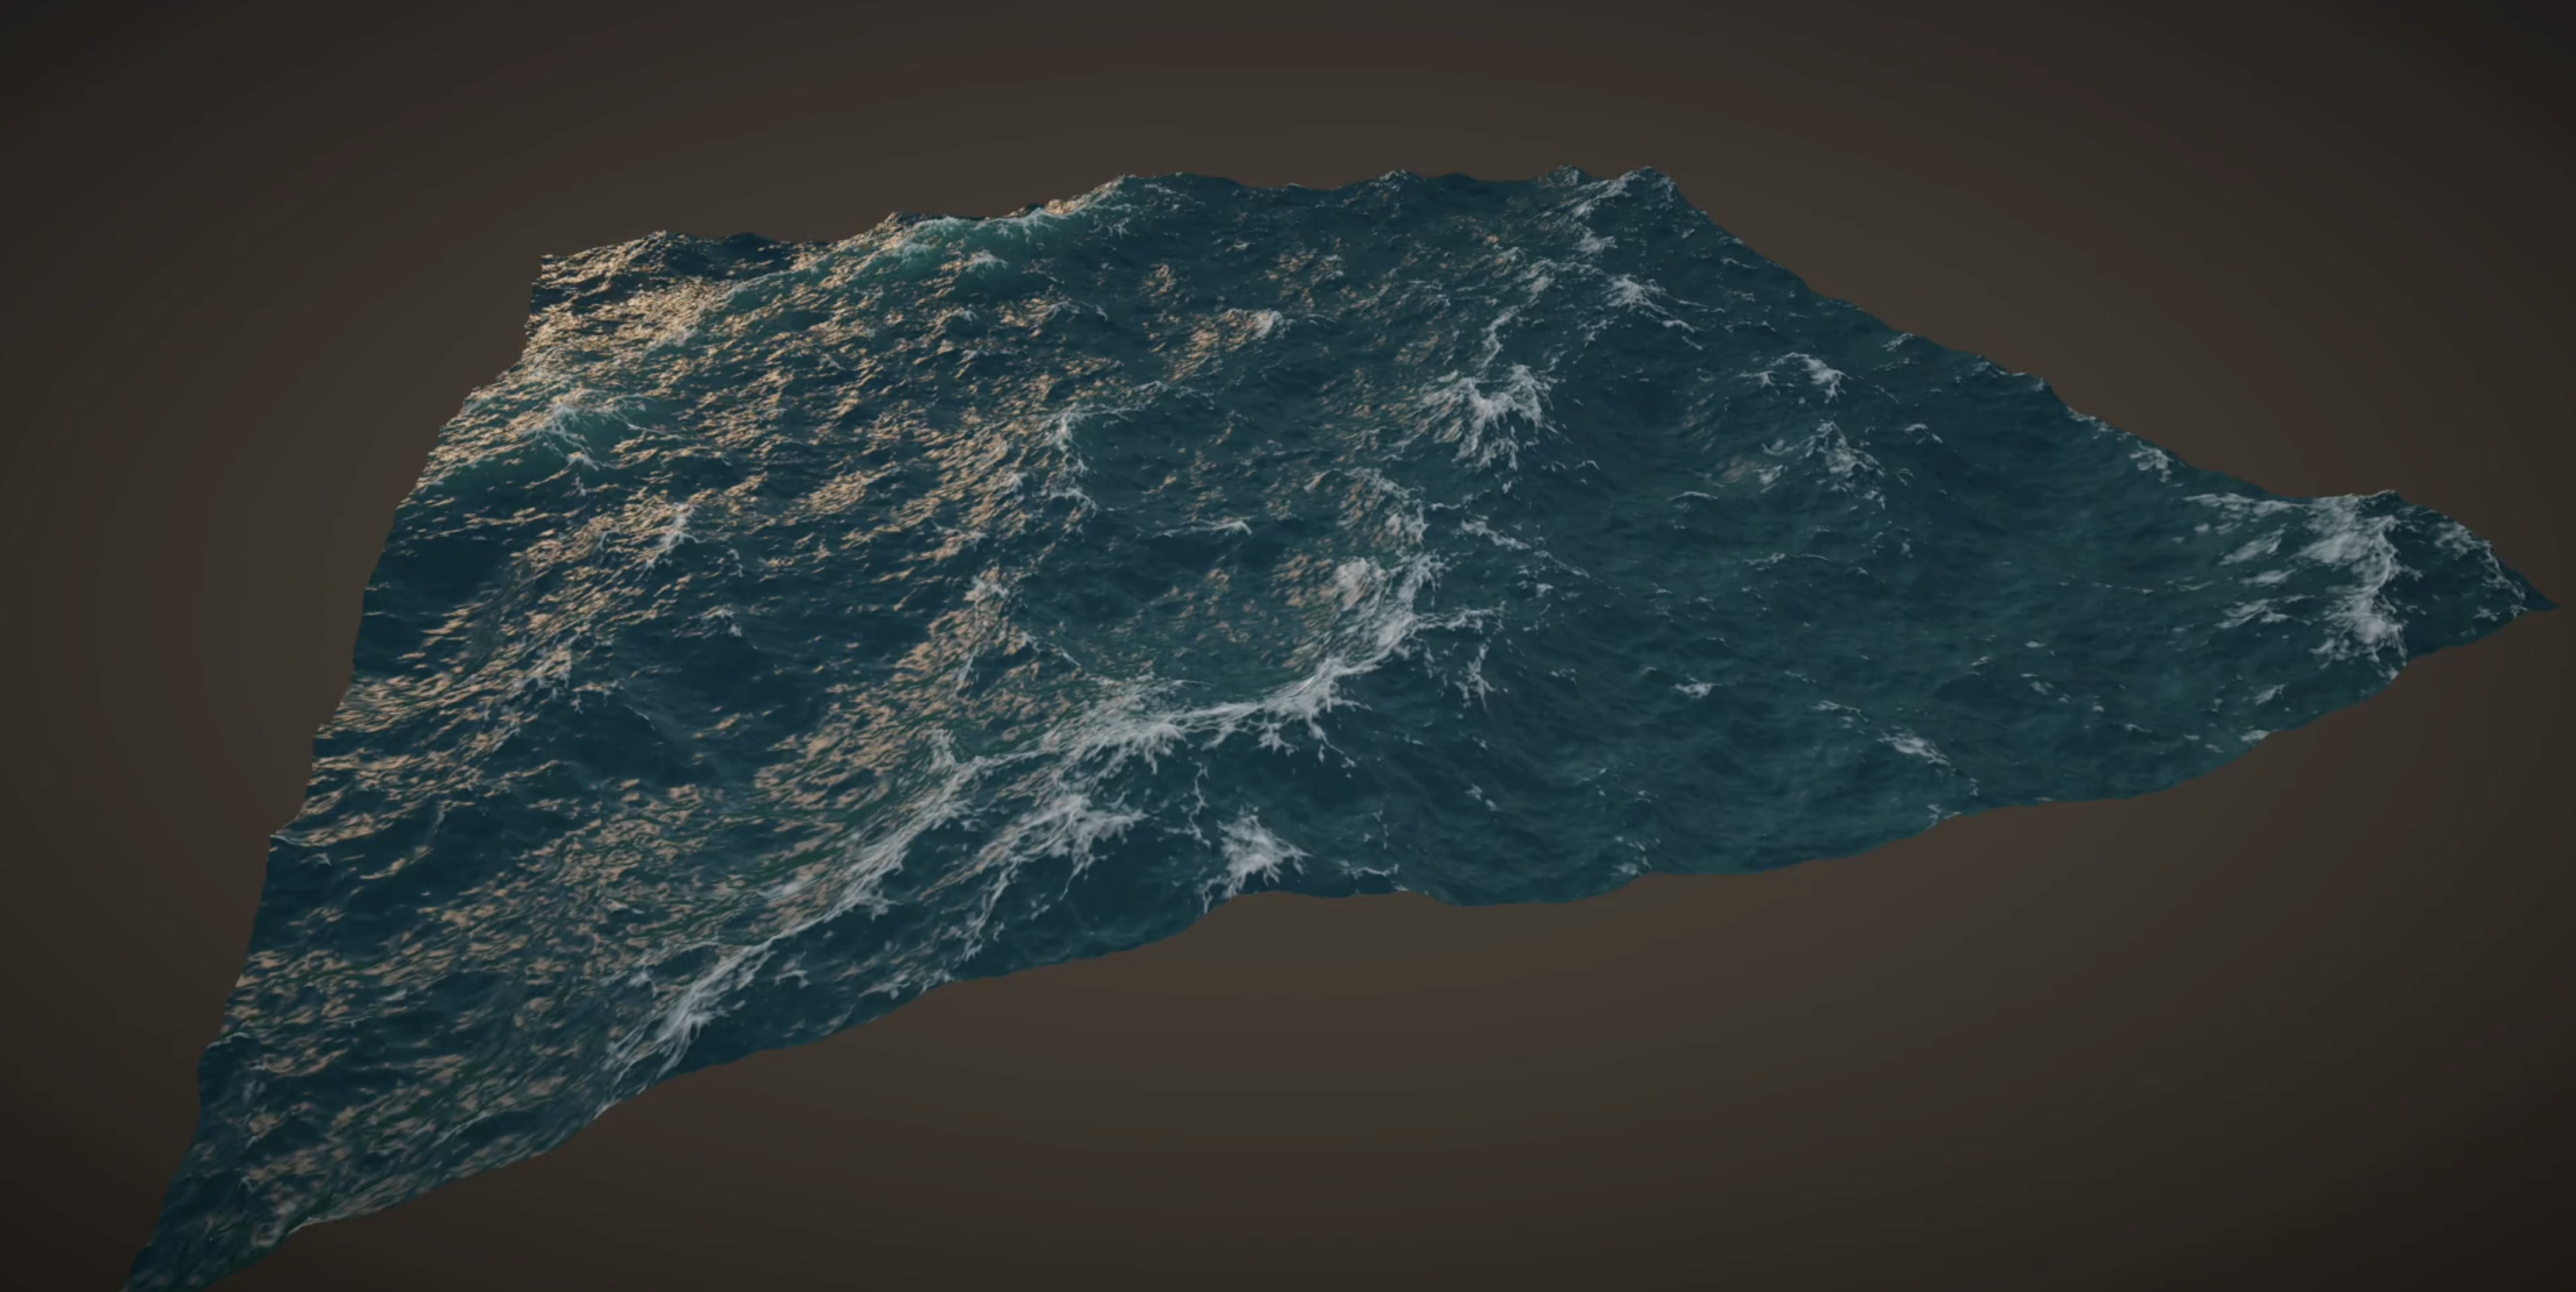
\includegraphics[width=0.8\textwidth]{"images/ocean_with_foam.png"}
    \captionof{figure}{Ocean With Foam}
    \label{fig:ocean_with_foam}
\end{minipage}

\section{Multiple Cascades}
At this stage our ocean with texture 512x512 simulates 262,144 distinc waves however the tilling is still noticible \ref{fig:ocean_with_tilling}.

\begin{minipage}{1\textwidth}
    \centering
    \includegraphics[width=0.8\textwidth]{"images/tilling_ocean.png"}
    \captionof{figure}{Ocean with Tilling, using 512x512 texture}
    \label{fig:ocean_with_tilling}
\end{minipage}

To counter this we could increase our simulation texture however even FFT becomes expensive really fast.
Another approuch is to simulate multiple cascades for diffrent wave lengths $k$ \ref{fig:cascades} and diffrent $l$ length scales. We can split our simulation into 3 parts, big waves, medium waves and small waves.

\begin{minipage}{1\textwidth}
    \centering
    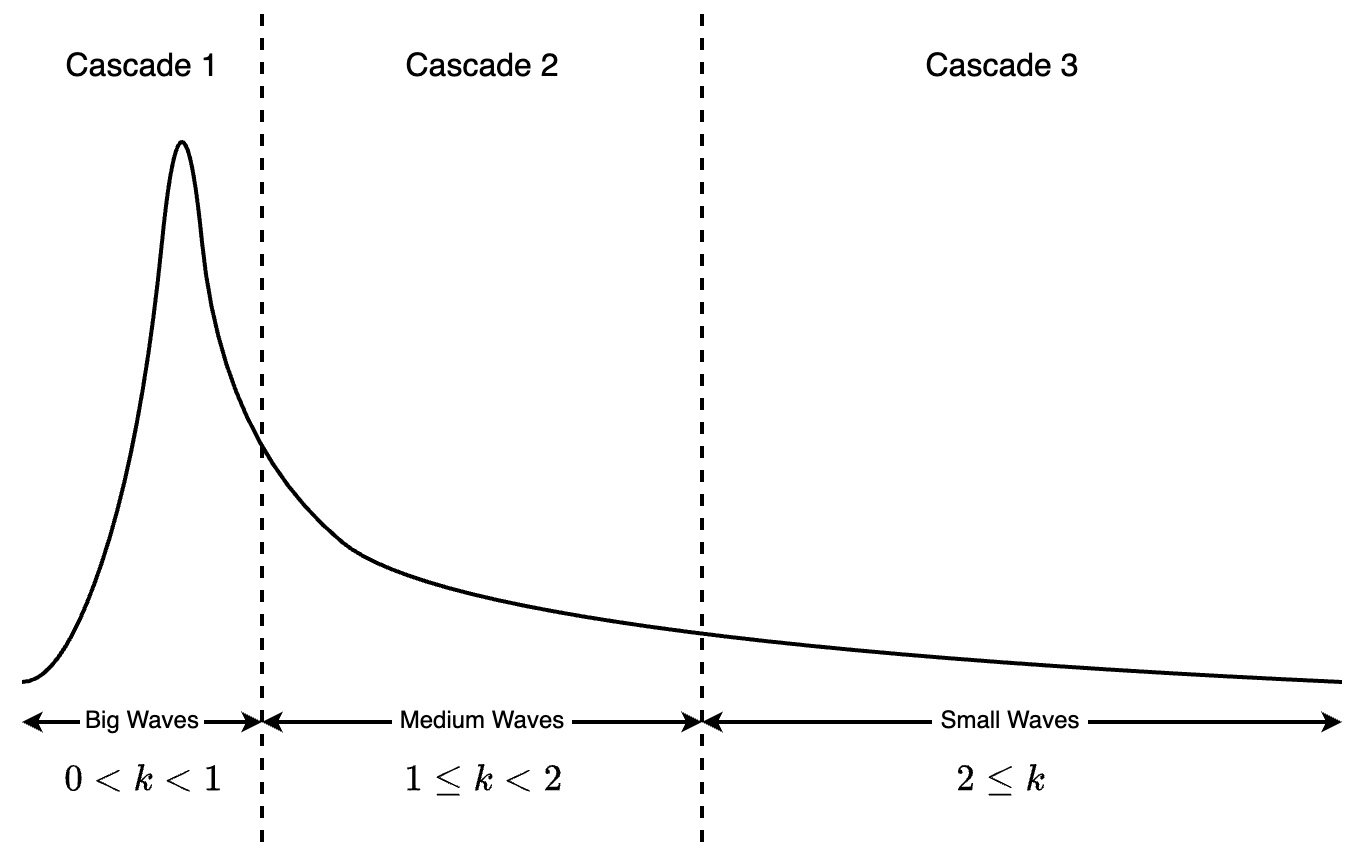
\includegraphics[width=0.8\textwidth]{"images/cascades.png"}
    \captionof{figure}{Cascades}
    \label{fig:cascades}
\end{minipage}
When it comes to chosing $l$ we need to follow these steps:
\begin{enumerate}
    \item We chose bigger $l$ for bigger waves as we are more likly to notice tilling with big waves
    \item We chose smaller $l$ for smaller waves as we are less likly to notice tilling with small waves
\end{enumerate}
This results ocean that has less tilling and more detail \ref{fig:ocean_with_cascades}.

\begin{minipage}{1\textwidth}
    \centering
    \includegraphics[width=0.8\textwidth]{"images/ocean_with_cascades.png"}
    \captionof{figure}{Ocean with Cascades, using 3x(512x512) textures}
    \label{fig:ocean_with_cascades}
\end{minipage}

One of the main pros of having multiple cascades is reduction in performance cost, as we can have similar results of 512x512 with 3x(256x256) xtextures as shown in figure \ref{fig:ocean_with_cascades_256}.

\begin{minipage}{1\textwidth}
    \centering
    \includegraphics[width=0.8\textwidth]{"images/ocean_cascades_256.png"}
    \captionof{figure}{Ocean with Cascades, using 3x(256x256) textures}
    \label{fig:ocean_with_cascades_256}
\end{minipage}

% Before we start, all callculations were taken inside GPU, using HLSL language. This allows us to use parallelism and speed up the process dramatically.
% As FFT requires our sample data length be power of 2, we will use $n \cdot n = 512 \text{x} 512$ textures to represent our data.

% \section{Spectrum Generation}
% \subsection{Tessendorf Spectrum}
% To generate height map \ref{eq:height_map} for our ocean we firstly need to generate spectrum. Firstlly, I chose to use J. Tessendorf's spectrum model \ref{eq:tessendorf_spectrum} as this was straight forward to implement:
% $$
% P_h(\mathbf{k}) = A \frac{e^{-1/(kl)^{2}}}{k^{4}}| \mathbf{\hat{k}} \cdot \mathbf{w} |^{6}
% $$
% where $\mathbf{k} = (k.x, k.y)$, $k.x = 2 * \pi (x.x - n/2)/ l$, $k.y = 2 * \pi (x.y - n/2)/ l$, $l$ is the the length scale of the ocean, 
% anx $\mathbf{x} = (x.x, x.y)$ is current position in the texture. 

% \subsection{TMA Spectrum}
% However, this model was not perfect, as it produced waves that didn't seem to transfer energy in the right way and the waves didn't seem to follow wave dircetion.
% Therefore, I decided to use JONSWAP spectrum with TMA correction that was suggested by \cite{horvath2015} \ref{eq:tma_spectrum}, however in our case $h$ will be constant therefore we can rewrite the function as:
% \begin{equation}
%     S_{TMA}(\omega) = S_{JONSWAP}(\omega) \cdot S_{TMA}(\omega)    
% \end{equation}
% Currentlly, we have two problems with this equation. Firstlly, this spectrum is non-directional, so we need to add directionality to it. Secondly, 
% this spectrum accepts $\omega$ as input, but as we following J. Tessendorf's \cite{tessendorf2001} paper, we need to use $\mathbf{k}$ as input. 

% \subsection{Directional Spectrum}



% According earlier expressed equation \ref{eq:height_map} we use DFT to calculate height map. Because we going to use FFT we can remove the exponential part as this will be calculated inside FFT algorithm:
% \begin{equation}
%     h(\mathbf{x}) = \sum_{\mathbf{k}} \tilde{h}(\mathbf{k}, t)
% \end{equation}
% , we can see that fft-based representation expresses ocean height at horizontal plane $\mathbf{x} = (x, y)$ "as the sum of sinusoids with complex, time-dependent amplitudes"\cite{tessendorf2001}.
% where, $\mathbf{k} = 2\pi $
